% !TeX root = ../main.tex

\chapter{討論}

兩種平坦隱沒模型各自的地質特徵有顯著不同。
本章將模型結果與觀測資料進行比對,討論兩種平坦隱沒類型之構造特色與岩漿作用狀態。
最後,將討論模型中影響平坦隱沒形成的可能原因。

\section{隱沒系統的耦合狀態}
隱沒板塊的耦合概念在1970年代晚期開始盛行(\citealp{uyeda1979back}; \citealp{ruff1980seismicity}),\citet{uyeda1979back}以隱沒板塊的年紀將隱沒帶分成兩種類型:第一種是年老隱沒板塊的馬尼亞納型(Mariana type)隱沒帶,第二種是年輕隱沒板塊的智利型(Chilean type)隱沒帶,示意圖如圖\ref{fig::end-member subduction}所示。
\begin{figure*}[htp]
    \centering
    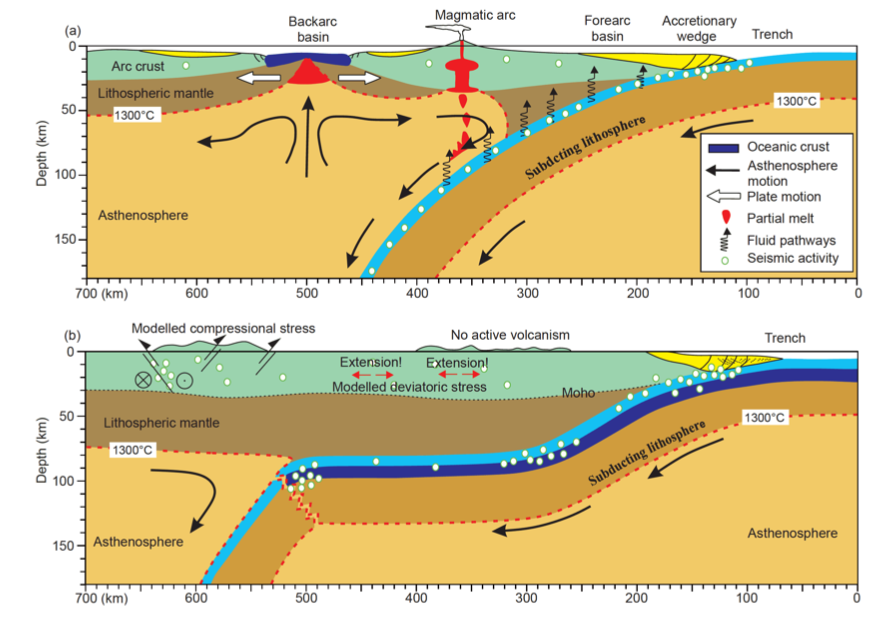
\includegraphics[width=6in]{2020subduction_type.png}
    \caption[隱沒帶的兩種型態示意圖,摘自\citet{Yan2020}]{隱沒帶的兩種型態示意圖,摘自\citet{Yan2020}。(a)馬尼亞納型隱沒帶(b)智利型隱沒帶}
    \label{fig::end-member subduction}
\end{figure*}

馬尼亞納型隱沒帶中隱沒板塊年紀較大、密度較大,重力較大造成隱沒板塊垂直分量上的拉力較大、隱沒傾角較高,與上覆板塊的接觸面積相對較小,可見圖\ref{fig::end-member subduction}a。
此類隱沒帶的應力不易累積,容易發生潛移活動,地震事件規模較小且通常為伸張地震,故馬尼亞納型隱沒帶又可稱為弱耦合(weak coupling)隱沒帶。
此外,高角度隱沒板塊易引起地函楔中強烈地函對流,伴隨隱沒帶部分熔融作用,在上覆板塊側發生拉張現象,可能會產生弧後張裂(back-arc spreading)(\citealp{lallemand2005relationships})。
反之智利型隱沒帶因隱沒板塊溫度較高、密度較小,故隱沒傾角較低,在聚合板塊交界處產生較大的板塊接觸面積,如圖\ref{fig::end-member subduction}b。
通常此類隱沒帶會容易產生低角度的班尼奧夫帶,地震事件多以逆衝斷層為主,且發生過多起大規模(Mw>8.0)地震事件(\citealp{uyeda1979back})。
上覆板塊側有顯著的壓縮應力(\citealp{hu2021southward}),可能會在弧後出現許多皺褶與斷層,因此智利型隱沒帶亦會被視為強耦合(strong coupling)隱沒帶。

\subsection{智利平坦隱沒的耦合狀態}
過去的研究注意到智利上覆板塊的地殼地震事件數目在平坦隱沒區域較多(\citealp{jordan1983andean}; \citealp{smalley1993basement}),表明平坦隱沒區域具有比正常隱沒帶更強的板塊間耦合。
\citet{gutscher2002andean}統計智利沿岸在距海溝250-800公里的所有地震事件所釋放之能量總和,以南北向一度以內為單位,獲得板塊釋放的地震能量直方圖(見圖\ref{fig::Chile_seismicity})。
總體而言,智利中部平坦隱沒上方的板塊所釋放出的地震能量比北部玻利維亞段高出5倍,比南段智利高出10倍。
\citet{jordan1983andean}分析智利沿岸大地震的震源機制解,顯示該區域以壓縮型地震主導,他認為隱沒邊界應力有效傳遞到上覆板塊,並且在平坦隱沒段有更高程度的板塊間耦合。

\begin{figure*}[htp]
    \centering
    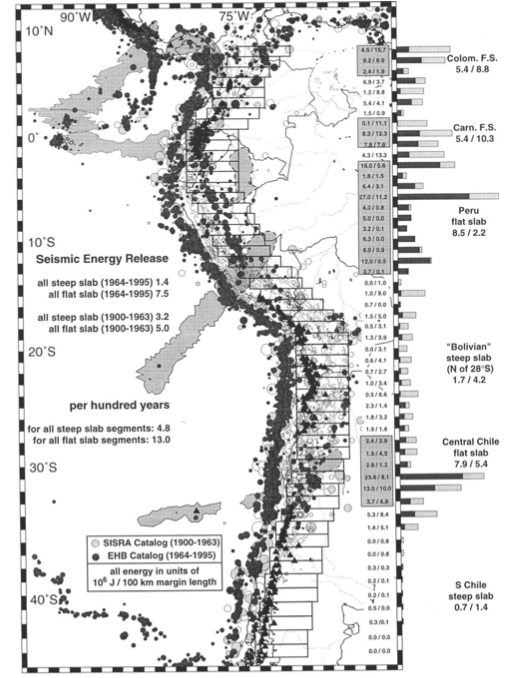
\includegraphics[width=5in]{Seismicity and Energy of Andes.png}
    \caption[智利沿岸自21$^\circ$S到44$^\circ$S的上板塊地震活動統計分析,摘自\citet{gutscher2002andean}]{智利沿岸自20$^\circ$S到40$^\circ$S的上板塊地震活動統計分析,摘自\citet{gutscher2002andean}。這裡採用深度<70公里的地震事件總能量,單位為10$^6$焦耳。右側數字表示1900-1963年/1964-1995年間所示分的地震能量。數字下灰色底框標示出平坦隱沒段的位置。
    }
    \label{fig::Chile_seismicity}
\end{figure*}

本研究智利參考模型的水平應力(Sxx)剖面圖如圖\ref{fig::Sxx_and_Pressure_Chile}a所示。
其中,水平應力大於0表示拉張,水平應力小於0表示壓縮。
上覆板塊側的水平應力在平坦隱沒段上地殼處有較小值,表示壓縮應力的存在。
上覆板塊的壓縮應力在水平方向上可分為兩區域,第一個區域位在近地表30公里以上、絕對座標550-650公里之間,其下方對應到隱沒板塊上凹變形處位置。
第二個區域較不明顯,位於絕對座標750-800公里、深度50-70公里處,對應到隱沒板塊下傾位置。
動水壓力剖面同樣可以觀察到類似的現象,在圖\ref{fig::Sxx_and_Pressure_Chile}b中,上覆板塊淺層於絕對座標550-650公里處有很大的正壓力,與圖\ref{fig::Sxx_and_Pressure_Chile}a中的壓縮應力位置相似。

\begin{figure*}[h]
    \centering
    \includegraphics[width=5.5in]{Sxx_and_Pressure_Chile_of_201.pdf}
    \caption[智利參考模型於40 Myr的水平軸差應力與動水壓力剖面]{智利參考模型於40 Myr的水平軸差應力與動水壓力剖面,其中應力正向代表拉張應力,負向代表壓縮應力。}
    \label{fig::Sxx_and_Pressure_Chile}
\end{figure*}

有趣的是,圖\ref{fig::Sxx_and_Pressure_Chile}a中平坦隱沒區上側、深度約100公里左右出現一段近150公里的拉張區,可能為板塊彎曲的結果,然而確切原因尚無論證。
\citet{comte2023anomalous}針對智利平坦隱沒區域的在2019年1月20日的板塊內地震事件進行餘震分析,發現在平坦隱沒頂部有多次正斷層事件發生,為拉張環境,與本研究結果相吻合。

\subsection{墨西哥平坦隱沒的耦合狀態}
墨西哥平坦隱沒並沒有強耦合的特徵。
\citet{PerezCampos2008}的接收函數結果顯示墨西哥的隱沒板塊平坦段深度直接位於莫荷面下方,因此隱沒板塊與上覆板塊的接觸面材質為海洋地殼與下部大陸地殼的成分,幾乎不包含任何大陸地函軟流圈(continental mantle asthenosphere),此時板塊介面在聚合過程中理論上應產生很大的摩擦力。
此外,墨西哥隱沒帶被視為侵蝕型隱沒(subduction erosion)(\citealp{stern2011subduction}),其證據包含現今外海的沉積物厚度約200公尺(\citealp{manea2003sediment}),並且擁有快速的聚合速率(\citealp{o2005uncertainties})。
再配合年輕隱沒帶的低傾角隱沒特徵,墨西哥平坦段聚合板塊接觸面積極大。
種種物理跡象表明該區域應該為強耦合環境。
然而墨西哥平坦隱沒段的地震活動度極低,格雷羅無震帶(\citealp{kostoglodov2003large})便位於平坦段上,表明平坦段並非處於強耦合狀態。
除此之外,平坦隱沒上方並沒有顯著的水平壓縮現象(\citealp{nieto2006latest}; \citealp{moran2007cenozoic}),這與強耦合的特徵互相矛盾。
對此,\citet{Manea2011Thermal}模擬墨西哥平坦隱沒剖面的熱構造。
隱沒板塊上海洋地殼與沉積物絕大部分在距海溝250公里前便完成脫水,大量的水分可能釋放進入下大陸地殼中,導致岩石強度降低,不容易累積大量應力。
該地區的非火山微震(non volcanic tremor)發生位置與海洋地殼的脫水位置相吻合\citet{Manea2011Thermal},慢地震(slow slip event)事件位置則與沉積物的脫水位置吻合\citet{Song2009}。
大量的微震與慢地震事件暗示著該區域為弱耦合隱沒帶。

本研究墨西哥參考模型的水平應力(Sxx)剖面圖如圖\ref{fig::Sxx_and_Pressure_Mexico}a所示。
上覆板塊側的水平應力在上部地殼與下部地殼底部各有一層高區。
此外,在絕對座標700公里與800公里處的火山島弧下方也具有地區性的水平應力小值,其為火山形成的荷重所造成。
與智利參考模型相比,墨西哥參考模型的上覆版塊沒有顯著的壓縮應力存在。
動水壓力剖面同樣可以觀察到類似的現象,如圖\ref{fig::Sxx_and_Pressure_Mexico}b所示,上覆板塊側除了上下地殼交界處與莫荷面處有較高的正壓力外,並沒有顯著來自隱沒板塊介面所提供的正壓力。
\begin{figure*}[ht!]
    \centering
    \includegraphics[width=5in]{Sxx_and_Pressure_Phase_Mexico_of_201_v5.pdf}
    \caption[墨西哥參考模型中於40 Myr的剖面]{墨西哥參考模型中於40 Myr的水平軸差應力、動水壓力與岩相剖面。(a)水平軸差應力剖面,其中應力正向代表拉張應力,負向代表壓縮應力。(b)動水壓力剖面。(c)模型岩相剖面,岩相顏色請見圖\ref{fig::Ref Cocos 26}。}
    \label{fig::Sxx_and_Pressure_Mexico}
\end{figure*}

本研究於第\ref{墨西哥隱沒帶地球物理觀測}節與第\ref{墨西哥參考模型結果}節皆有提及地震學研究在墨西哥平坦隱沒區域的板塊介面中發現一層低速層(\citealp{PerezCampos2008}),\citealp{Song2009}估計該低速層厚度約3-5公里且V$_S$速度約每秒2-2.7公里,大約降低26-40$\%$左右。
過去對於該低速層的成分有諸多解釋,\citet{Song2012SC}認為其為經歷強烈剪切的變質岩成分。
\citet{Manea2017}則認為該弱耦合物質為殘餘的蛇紋岩。

從墨西哥參考模型的岩相圖\ref{fig::Sxx_and_Pressure_Mexico}c可見隱沒板塊與大陸地殼的介面中具有厚度4-8公里、以沉積岩為主參雜少許蛇紋岩化橄欖岩的弱物質。
由於該弱物質層的岩石強度極弱,故隱沒板塊介面成為弱耦合介面,上覆板塊的壓縮應力較小。
因此,並非所有低傾角隱沒帶皆具有強耦合的特徵。

\section{平坦隱沒中的埃達克岩}\label{平坦隱沒中的埃達克岩}
埃達克岩(adakite)最初由\citet{kay1978aleutian}觀測阿留申群島中Adak Island上一種高La/Yb、高Sr/Y以及富含大離子半徑元素(large ion lithophile (LIL)- element-rich)的安山岩,其特徵與一般的火山島弧安山岩不相同,爾後\citet{defant1990derivation}將其命名為埃達克岩。
由於埃達克岩具有特殊的全岩地球化學性質,一般多半利用Sr/Y-Y作圖與(La/Yb)$_N$-Yb$_N$作圖區別埃達克岩與一般的島弧中酸性安山岩,如圖\ref{fig::AdakiteY}。

\begin{figure*}[h]
    \centering
    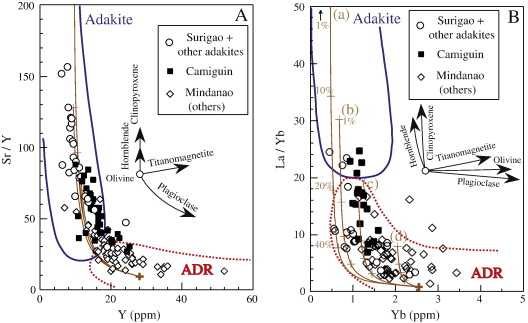
\includegraphics[width=5in]{AdakiteY.jpg}
    \caption[Sr/Y-Y作圖與(La/Yb)$_N$-Yb$_N$作圖]{(A)Sr/Y-Y作圖與(B)(La/Yb)$_N$-Yb$_N$作圖,摘自\citet{castillo2012adakite}。通常用於區分埃達克岩與普通島弧安山岩、石英岩與流紋岩(normal arc andesite, dacite and rhyolite, ADR)。紫色實線邊界來自於\citet{richards2007special}所提出菲律賓中南部埃達克岩與普通島弧安山岩的資料。}
    \label{fig::AdakiteY}
\end{figure*}

早期認為埃達克岩是年輕的(< 7 Ma)隱沒海洋玄武岩發生部分熔融產生的中酸性火山岩(\citealp{defant1990derivation}; \citealp{peacock1994partial})。
由於埃達克岩的定義來自岩石化學組成分定量分析,隨著相關研究累積,顯示高壓變質基性岩的部分熔融皆具有埃達克岩的特徵,
因此埃達克岩性質的火成岩可以在多種不同地體環境下產生(\citealp{martin2005overview}),以下列出最常見的四種:

(1)隱沒海洋地殼的熔融(\citealp{defant1990derivation}),隨後埃達克岩中的低Nd、高Sr同位素特徵被認為是隱沒海洋沉積物參與部分熔融所產生(\citealp{stern1996role}; \citealp{gomez2003temporal}),又有人稱其為high-SiO$_2$ adakites (\citealp{martin2005overview})。

(2)增厚大陸下地殼底部的基性岩熔融(\citealp{kay1996magmatic})。
在高壓環境下,基性岩密度過高時無法穩定存在於大陸地殼底部,因此部分熔融產生。
通常需要長時間的地殼增厚(\citealp{kay2002magmatism})才會形成高壓下的高密度基性岩,因此這種形成機制比較可能會發生在島弧岩漿作用事件中末期。

(3)普通島弧安山岩受地殼成分污染,導致岩漿混合,其稱為low-SiO$_2$ adakites (\citealp{martin2005overview}),與(1)成因中的high-SiO$_2$ adakites相對。
此埃達克岩具有較高的地函組成相關元素(MgO、K、Nb、Cr、Ni等)。

(4)來自一般的島弧基性岩漿於高壓(> 12 kbar)環境下,以石榴子石為主的結晶分化產物(\citealp{moyen2009high}),例如菲律賓蘇里高半島的埃達克岩。

一般來說,上述成因中,只有(1)與(2)兩種成因可被稱為埃達克岩,而(3)與(4)所產生之高Sr/Y類似因物質交換而繼承埃達克岩特徵,稱作類埃達克岩(Adakite-like rocks)(\citealp{kay2002magmatism}; \citealp{goss2013andean})。

早期在南美洲的平坦隱沒區域發現部分埃達克岩的紀錄,\citet{Gutscher2000Bcan}為此提出一概念模型,為平坦隱沒特殊的溫壓條件所生成埃達克岩。
如同\ref{墨西哥參考模型脫水位置與岩漿作用}節所提及,平坦隱沒具有與正常隱沒帶不同的溫壓路徑,如圖\ref{fig::Flat slab PT}中所繪,此時鐵鎂岩相與沉積岩相很有可能會通過固熔點,導致海洋地殼發生部分熔融。

\begin{figure*}[ht!]
    \centering
    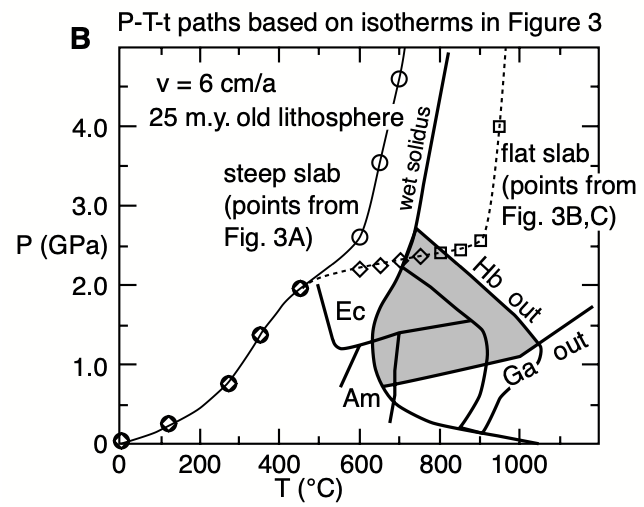
\includegraphics[width=4in]{Flat slab PT.png}
    \caption[隱沒板塊頂部可能的溫壓路徑圖,摘自\citet{Gutscher2000Bcan}]{隱沒板塊頂部可能的溫壓路徑圖,摘自\citet{Gutscher2000Bcan}。Ec—榴輝岩(eclogite),Am—角閃岩(amphibolite),Ga—石榴石(garnet),Hb—角閃石(hornblende)。
    圓形為正常隱沒帶中的溫壓路徑,菱形與正方形則為平坦隱沒的溫壓路徑。其中,灰色底部分為隱沒板塊可能的部分熔融區。
    }
    \label{fig::Flat slab PT}
\end{figure*}

\subsection{墨西哥平坦隱沒的岩漿作用}
在墨西哥,地球化學上所認定的埃達克岩的特徵之一為高Gd/Yb與高SiO$_2$,如圖\ref{fig::Cocos_geochemisty}b與圖\ref{fig::Cocos_geochemisty}c所示。
跨墨西哥火山帶最初於早中新世(約19 Ma)開始噴發,主要為亞鹼性(sub-alkaline)岩石,由安山岩和英安岩組成,隨著火成岩噴發位置離海溝越來越遠,地球化學特徵表明越往北(遠離海溝)的火成岩,隱沒帶中的流體量越少(\citealp{ferrari2012dynamic})。
這個趨勢在15 Ma左右被侵入的埃達克岩中斷(\citealp{mori2007effects}),見圖\ref{fig::Cocos_geochemisty}a紅色與藍色點,值得注意的是,具有埃達克岩特徵的樣本幾乎都與海溝距離超過400公里。
目前學界一致認同墨西哥平坦隱沒區域所發現的埃達克岩樣本皆為隱沒海洋地殼與沉積物的產物(\citealp{Gutscher2000Bcan}; \citealp{ferrari2012dynamic}; \citealp{Manea2017})。

\begin{figure*}[ht!]
    \centering
    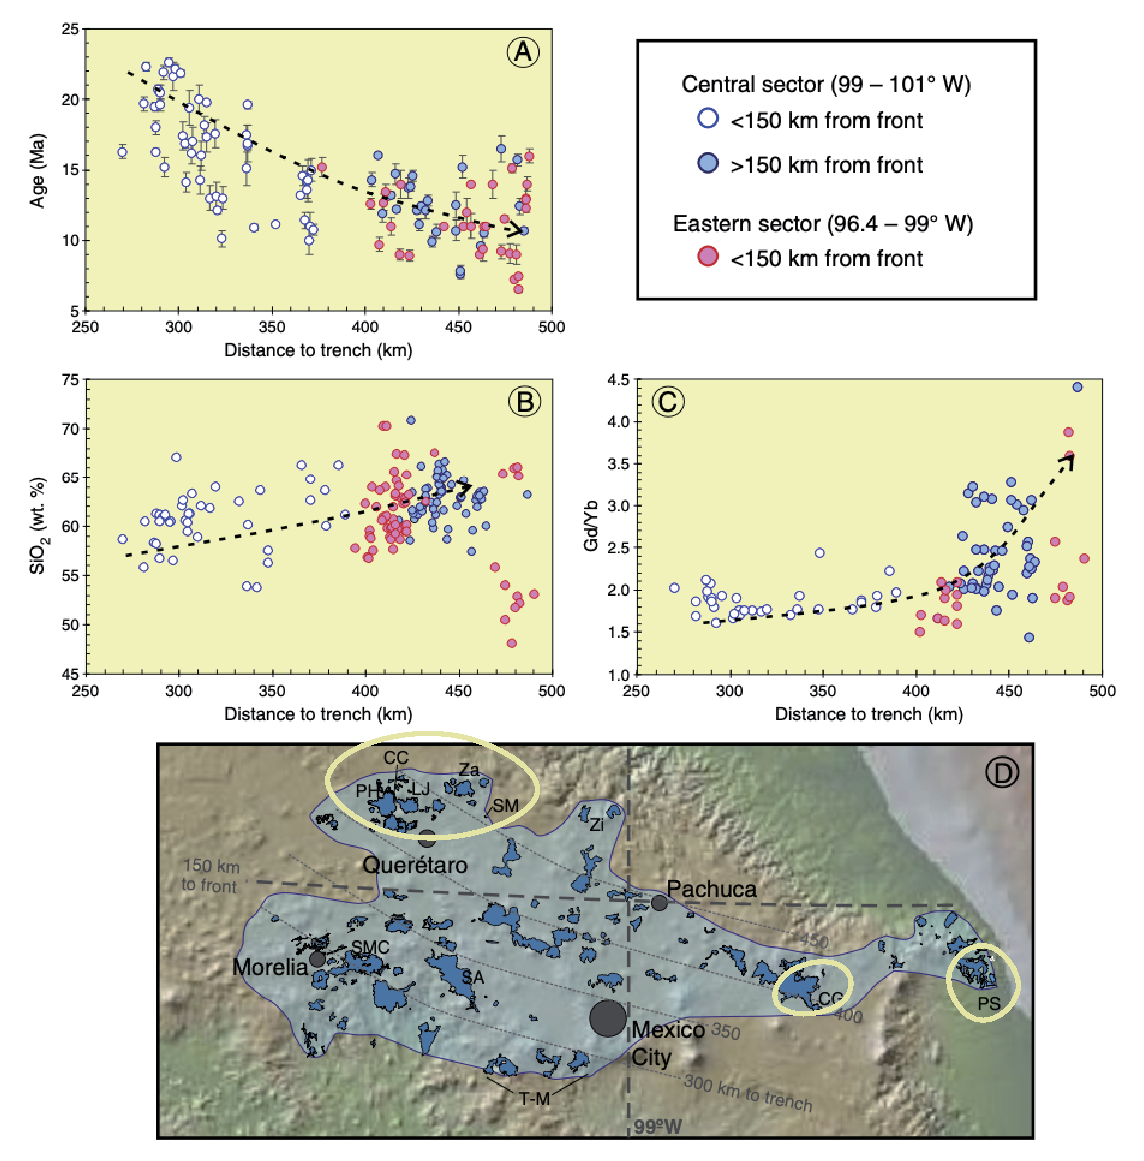
\includegraphics[width=5in]{Cocos_Volcano_v2.pdf}
    \caption[墨西哥區域火山島弧地球化學分析,摘自\citet{ferrari2012dynamic}]{墨西哥區域火山島弧地球化學分析,摘自\citet{ferrari2012dynamic}。白點為距現今火山弧前緣小於150公里的樣本,藍色點為具現今火山弧前緣大於150公里且位在西經99-101$^{\circ}$的樣本,紅色點為具現今火山弧前緣小於150公里且位在西經96.4-99$^{\circ}$的樣本。(a)火成岩樣本年紀與現今海溝距離作圖。(b)火成岩樣本中的SiO$_2$含量與現今海溝距離作圖。(c)火成岩樣本中Gd/Yb比值與現今海溝距離作圖。(d)墨西哥中新世火山位置圖。細虛線表示到海溝的距離,粗虛線是\ref{平坦隱沒中的埃達克岩}圖例中使用的邊界。 CC: Cerro Colorado dome,CG: Cerro Grande volcan塞羅格蘭德火山, LJ: La Joya volcan拉霍亞火山, PH: Palo Huérfano 火山, PS: Palma Sola帕爾馬索拉,SA: Sierra de Angangueo塞拉利昂德安甘格奧, SM: San Martín聖馬丁, SMC: Sierra de Mil Cumbres, T-M: Tenancingo–Malinalco特南寧哥-馬利納爾科, Za: Zamorano volcano薩莫拉諾火山, Zi: Zimapán area Zimapán 地區。
    }
    \label{fig::Cocos_geochemisty}
\end{figure*}

在墨西哥參考模型中,確實有海洋地殼部分熔融的現象。
圖\ref{fig::Cocos Ref melting time}b、c中顯示平坦隱沒形成、於模型時間15 Myr前後開始發生榴輝岩的部分熔融。
榴輝岩的部分熔融比例在平坦隱沒形成初期快速增加,在15-20 Myr之間可達50-70$\%$。
在20 Myr後,榴輝岩的部分熔融比例維持5-20$\%$之間,在時間軸上沒有太大改變。
然而沉積物自23 Myr後便成為墨西哥參考模型熔融源的主導岩石。
儘管多數研究已證實隱沒沉積物大量熔融的存在(\citealp{van2011subduction}; \citealp{Forster2021}),本研究認為該結果需要進一步確認。
本研究中,所選用的沉積物固相線為飽和水固相線(\citealp{van2011subduction}),然而模型中並沒有考量各岩石的含水量多寡,因此部分熔融的形成機制需要更多考量。

\citet{stern1996role}針對埃達克岩樣本進行分析,表示埃達克岩中約有35-90$\%$的隱沒板塊質量,包含玄武岩、榴輝岩與沉積物。
圖\ref{fig::melting_eclogite_ratio}是墨西哥參考模型在時間軸上岩漿熔融源與熔融量變化圖,只關注於平坦隱沒發生後的岩石熔融。
圖\ref{fig::melting_eclogite_ratio}b顯示模型中榴輝岩的熔融比例與岩漿庫體積,在平坦隱沒剛形成時(15-20 Myr),所有熔融岩中,有超過40$\%$為榴輝岩,爾後榴輝岩體積比例維持10-20$\%$。
由於本研究並沒有考慮大陸地殼中的岩漿作用,以及岩漿內物質置換、結晶分異作用與岩石含水量對岩漿庫的影響,因此無法充分說明模型中所產生的火山島弧是否確切為埃達克岩的成分。
然而從模型中岩漿作用熔融源分析可證明(見圖\ref{fig::melting_eclogite_ratio}a),隱沒板塊物質確實可以發生熔融。

圖\ref{fig::Mexico_arc_location}顯示墨西哥參考模型中地表出現兩處的火山島弧。
第一處的火山島弧出現於距海溝130-180公里處,可以對應至圖\ref{fig::Cocos Ref 2Dtime series}b中的第二區岩漿庫(Magma Chamber 2)。
第二處的火山島弧出現於距海溝260-280公里處,可以對應至圖\ref{fig::Cocos Ref 2Dtime series}b中的第三區岩漿庫(Magma Chamber 3)。
本研究所產生的火山島弧與海溝距離不及圖\ref{fig::Cocos_geochemisty}中的墨西哥火山島弧,不過確實可獲得沿海溝距離上火成岩成分的劇烈變化結果。

\begin{figure*}[ht!]
    \centering
    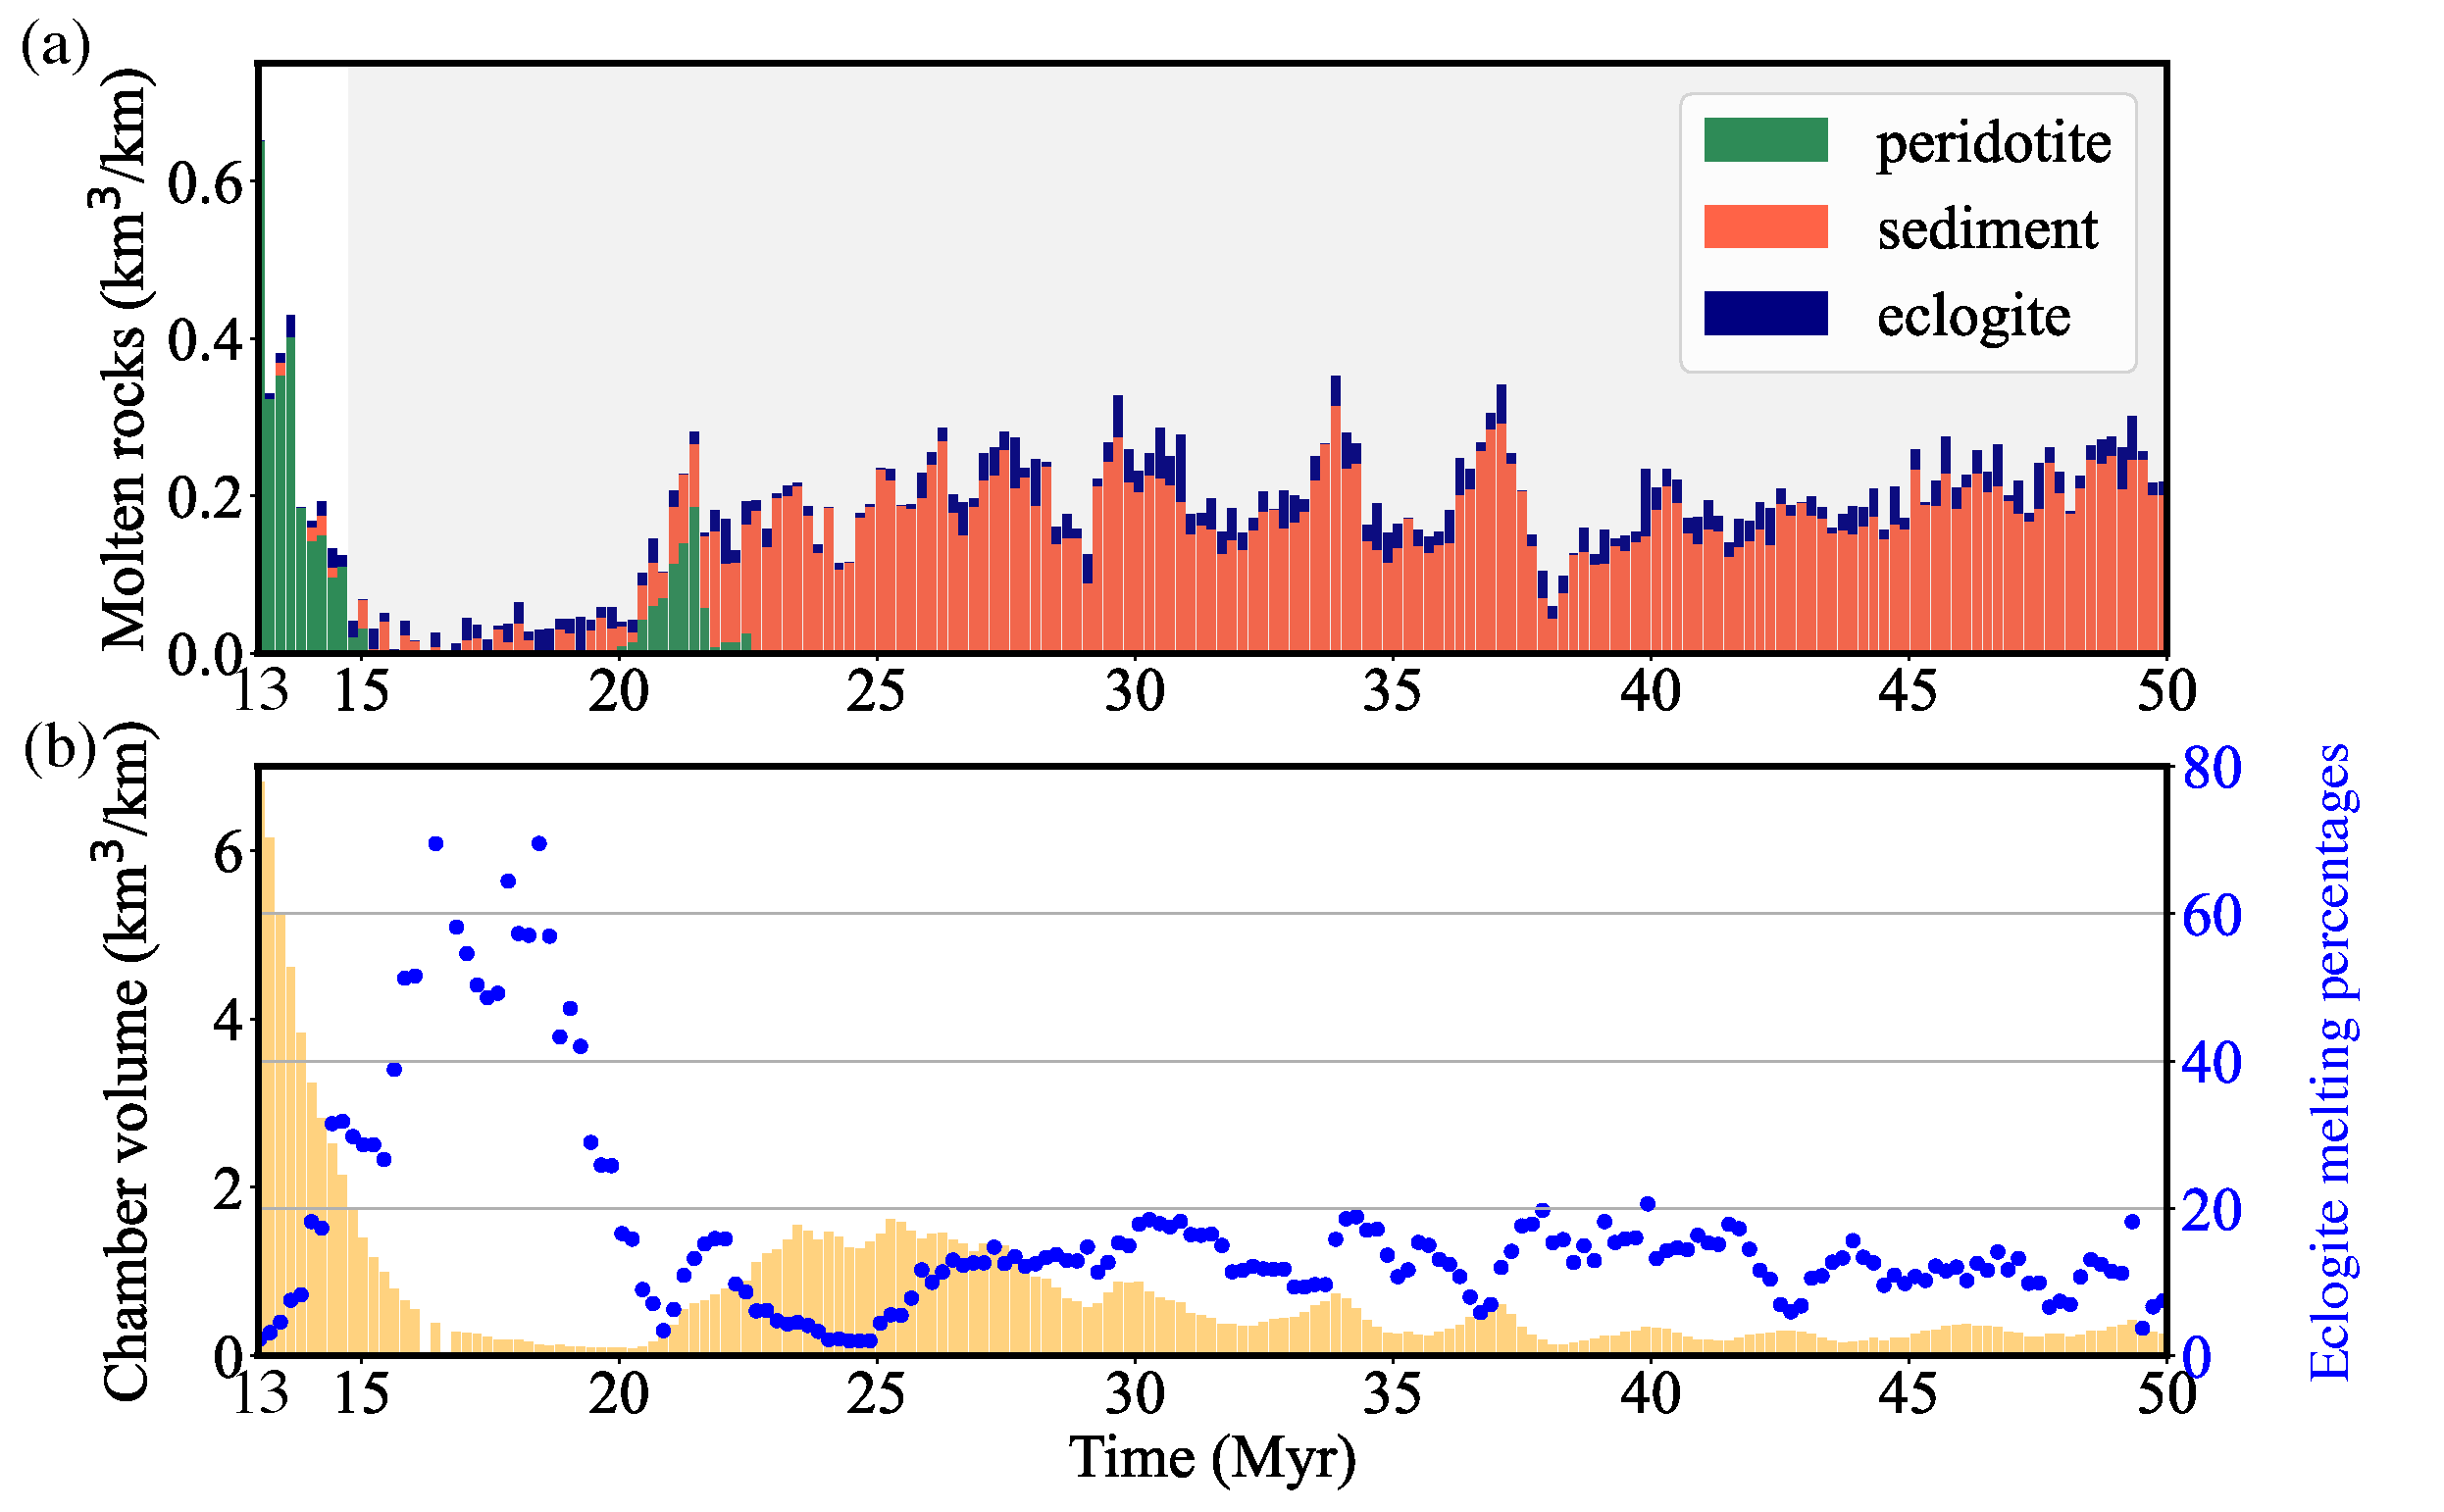
\includegraphics[width=6in]{slab_melting.pdf}
    \caption[墨西哥參考模型部分熔融源岩與岩漿庫分析]{墨西哥參考模型部分熔融源岩與岩漿庫分析。(a)同圖\ref{fig::Cocos Ref melting time}b,聚焦在13-40 Myr時期的部分熔融源岩,熔融量單位為每單位海溝產生之立方公里量中每20萬年瞬時量,模型中包含橄欖岩(綠色)、沉積岩(橘色)與榴輝岩(深藍色)熔融。灰底為平坦隱沒發生時間。(b)黃底柱狀為岩漿庫體積,藍點為榴輝岩瞬時熔融體積佔整體瞬時熔融體積的比例。
    }
    \label{fig::melting_eclogite_ratio}
\end{figure*}

\begin{figure*}[ht!]
    \centering
    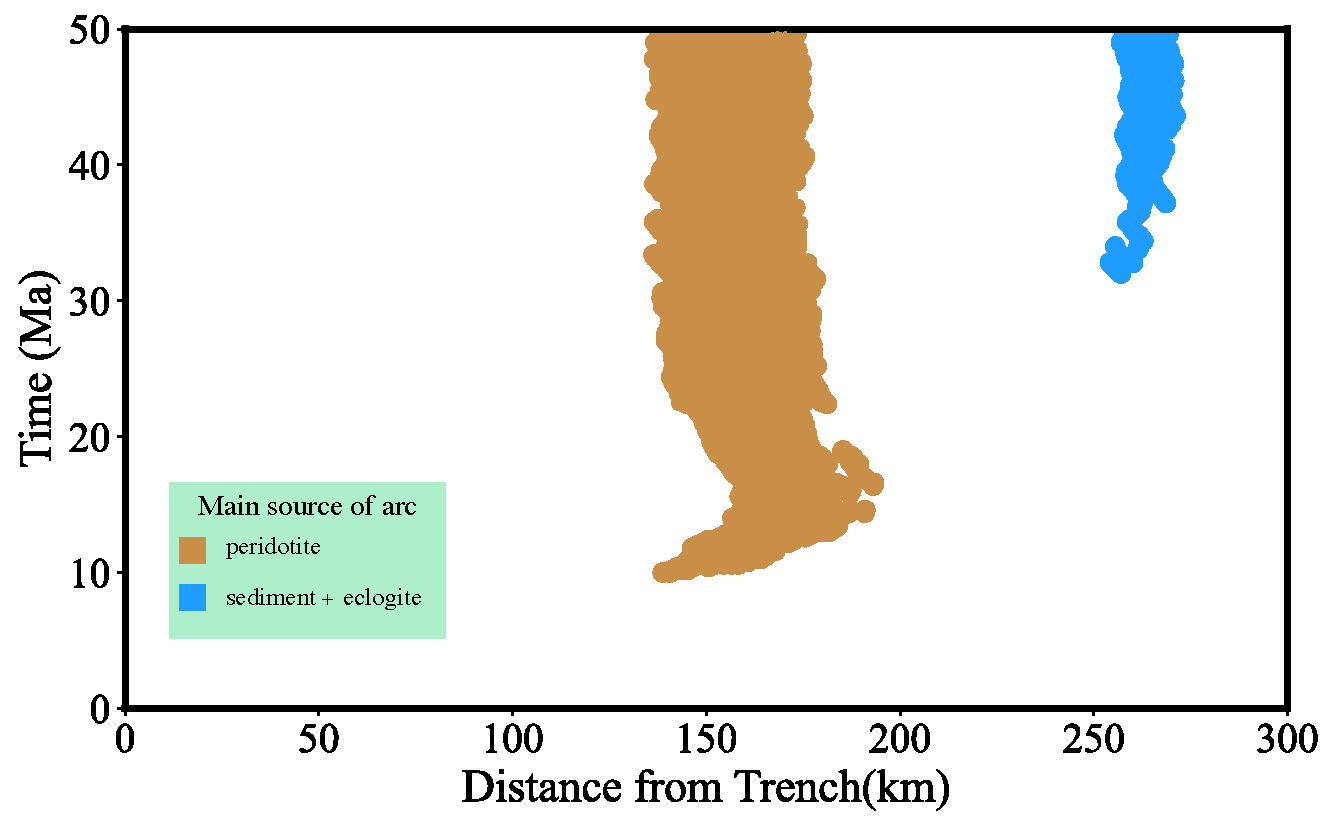
\includegraphics[width= 5in]{Mexico_arc_location_v1.pdf}
    \caption[墨西哥參考模型火山島弧與海溝距離隨時間變化]{墨西哥參考模型火山島弧與海溝距離隨時間變化。其中咖啡色為熔融源岩以橄欖岩為主的火山島弧,藍色則為熔融源岩以沉積物與榴輝岩為主的火山島弧。
    }
    \label{fig::Mexico_arc_location}
\end{figure*}

\newpage
\subsection{智利平坦隱沒的岩漿作用}

\citet{Gutscher2000Bcan}認為南美洲平坦隱沒區域所出露的埃達克岩為隱沒板塊熔融的產物,在他們的研究中僅使用概念模型解釋埃達克岩成因,然而\citet{kay2002magmatism}近一步對埃達克岩樣本進行地球化學分析,他們認為智利區域的埃達克岩為上述成因中的第(3)種,埃達克岩漿來自於普通島弧安山岩漿與地殼熔融發生岩漿混合,是為low-SiO$_2$ adakites。
由於本研究並沒有考慮大陸地殼成分岩石發生部分熔融,因此無法從參考模型中獲得\citet{kay2002magmatism}所認為的結果。
然而,將智利參考模型隱沒地殼頂部溫壓狀態與隱沒板塊相圖比較(見圖\ref{fig::chile_slab_PT}),隱沒板塊並沒有通過隱沒板塊含水固相線。
此外,智利參考模型的平坦深度在100公里左右,圖\ref{fig::chile_slab_PT}中壓力維持不變且溫度持續增加的範圍落在3 GPa與攝氏500-800 $^{\circ}$之間,圖\ref{fig::Flat slab PT}中\citet{Gutscher2000Bcan}的概念模型平坦段範圍落在2.5 GPa與攝氏400-900$^{\circ}$,兩者有顯著差異。
以智利平坦隱沒區的平坦段深度100公里來看,智利參考模型的結果較接近真實情形。
這說明本研究可排除\citet{Gutscher2000Bcan}中所認為的埃達克岩形成方式。

\begin{figure*}[ht!]
    \centering
    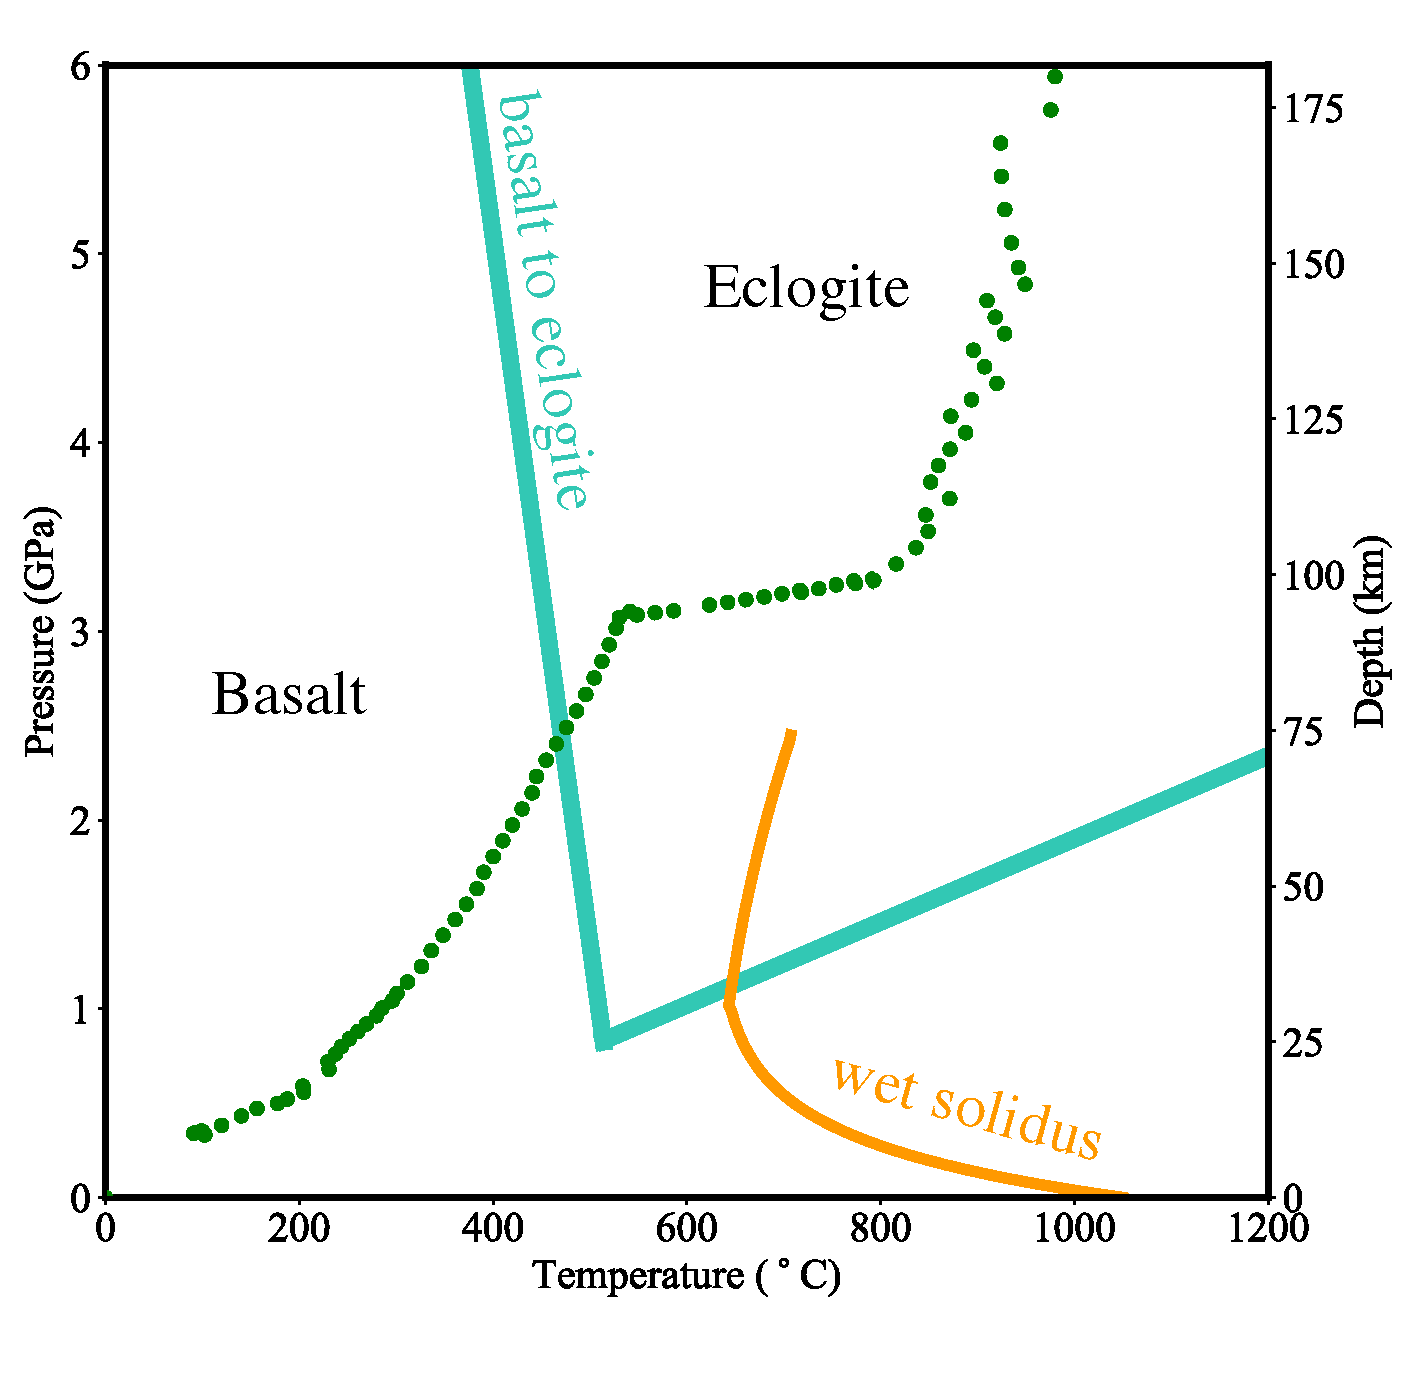
\includegraphics[width=4in]{chile_slab_PT_v1.pdf}
    \caption[智利參考模型隱沒地殼頂部於40 Myr的溫壓圖]{智利參考模型隱沒地殼頂部於40 Myr的溫壓圖。其中綠線為本研究中玄武岩至榴輝岩的相變條件,橘色線為含水固相線。綠色點為隱沒地殼頂部每2-5公里的溫壓狀態。
    }
    \label{fig::chile_slab_PT}
\end{figure*}

\newpage
\section{為什麼會形成平坦隱沒}
由於平坦隱沒的形成原因至今依然是一開放性問題,以下將討論隱沒帶中不同構造區對隱沒系統的影響,以及本研究模型中產生平坦隱沒的可能關鍵原因。
本節測試一系列數值模型參數,模型參數表見表\ref{模型參數列表}。

\begin{table}[htp]\large
    \caption[模型參數列表]{模型中參數列表}
    \label{模型參數列表}
    \renewcommand{\arraystretch}{1.2}
    \centering
    \begin{tabular}{|lllll|}
        \hline
        \multicolumn{5}{|c|}{Upper Plate Thickness}                                                 \\ \hline
        model        & P$_0$                   & $\lambda_0$             & thickness & serpentinite \\ \hline
        Nazca\_a01 & 4.5 $\times$ 10$^{-15}$ & 1.6 $\times$ 10$^{-12}$ & 120       & 5            \\
        Ref\_Nazca   & 4.5 $\times$ 10$^{-15}$ & 1.6 $\times$ 10$^{-12}$ & 130       & 5            \\
        Nazca\_a02 & 4.5 $\times$ 10$^{-15}$ & 1.6 $\times$ 10$^{-12}$ & 140       & 5            \\
        Nazca\_a03 & 4.5 $\times$ 10$^{-15}$ & 1.6 $\times$ 10$^{-12}$ & 150       & 5            \\
        Nazca\_a04 & 4.5 $\times$ 10$^{-15}$ & 1.6 $\times$ 10$^{-12}$ & 160       & 5            \\ \hline
        \multicolumn{5}{|c|}{Serpentinite Thickness}                                                \\ \hline
        model        & P$_0$                   & $\lambda_0$             & thickness & serpentinite \\ \hline
        Nazca\_b01 & 4.5 $\times$ 10$^{-15}$ & 1.6 $\times$ 10$^{-12}$ & 130       & 2.5          \\
        Ref\_Nazca   & 4.5$\times$ 10$^{-15}$  & 1.6 $\times$ 10$^{-12}$ & 130       & 5            \\
        Nazca\_b02 & 4.5 $\times$ 10$^{-15}$ & 1.6 $\times$ 10$^{-12}$ & 130       & 7.5          \\
        Nazca\_b03 & 4.5 $\times$ 10$^{-15}$ & 1.6 $\times$ 10$^{-12}$ & 130       & 10           \\
        Nazca\_b04 & 4.5 $\times$ 10$^{-15}$ & 1.6 $\times$ 10$^{-12}$ & 130       & 15           \\ \hline
        \multicolumn{5}{|c|}{Magma Parameters}                                                      \\ \hline
        model        & P$_0$                   & $\lambda_0$             & thickness & serpentinite \\ \hline
        Ref\_Nazca   & 4.5 $\times$ 10$^{-15}$ & 1.6 $\times$ 10$^{-12}$ & 130       & 5            \\
        Nazca\_c01 & 4.5 $\times$ 10$^{-14}$ & 1.6 $\times$ 10$^{-12}$ & 130       & 5            \\
        Nazca\_c02 & 4.5 $\times$ 10$^{-13}$ & 1.6 $\times$ 10$^{-12}$ & 130       & 5            \\
        Nazca\_c03 & 4.5 $\times$ 10$^{-15}$ & 1.6 $\times$ 10$^{-13}$ & 130       & 5            \\
        Nazca\_c04 & 4.5 $\times$ 10$^{-14}$ & 1.6 $\times$ 10$^{-13}$ & 130       & 5            \\
        Nazca\_c05 & 4.5 $\times$ 10$^{-13}$ & 1.6 $\times$ 10$^{-13}$ & 130       & 5            \\
        Nazca\_c06 & 4.5 $\times$ 10$^{-15}$ & 1.6 $\times$ 10$^{-14}$ & 130       & 5            \\
        Nazca\_c07 & 4.5 $\times$ 10$^{-14}$ & 1.6 $\times$ 10$^{-14}$ & 130       & 5            \\
        Nazca\_c08 & 4.5 $\times$ 10$^{-13}$ & 1.6 $\times$ 10$^{-14}$ & 130       & 5            \\
        Nazca\_c09 & 4.5 $\times$ 10$^{-15}$ & 1.6 $\times$ 10$^{-15}$ & 130       & 5            \\
        Nazca\_c10 & 4.5 $\times$ 10$^{-14}$ & 1.6 $\times$ 10$^{-15}$ & 130       & 5            \\
        Nazca\_c11 & 4.5 $\times$ 10$^{-13}$ & 1.6 $\times$ 10$^{-15}$ & 130       & 5            \\ \hline
    \end{tabular}
\end{table}

\subsection{均質的隱沒板塊}
本研究的兩種參考模型中,隱沒板塊上皆不存在任何非均質(heterogeneous)構造或任何例外的物理特性。
同\ref{平坦隱沒的數值模型}所述,過去的數值模型提出許多降低隱沒系統重力力矩的可能原因,包含加入一段不會發生玄武岩相變的海洋地殼(\citealp{Liu2016}; \citealp{Gerya2009})、延後榴輝岩相的相變時間(\citealp{van2002role})、增厚隱沒海洋地殼(\citealp{Liu2016}; \citealp{axen2018basal})、降低整體隱沒岩石圈密度(\citealp{Gerya2009})以及設計隱沒板塊隱沒後斷裂(\citealp{Liu2016}; \citealp{axen2018basal})等。

早期研究認為隱沒的海洋高原最有可能是平坦隱沒的形成原因(\citealp{gutscher2002andean})。
\citet{Skinner2013}利用磁力條帶重建納茲卡板塊上海洋高原及洋脊位置,並且計算其隱沒進入南美板塊的時間。
他們的研究表明隱沒的地殼增厚體與平坦隱沒發生時間錯開,因此平坦隱沒的形成原因可能無法完美的被地殼增厚體所解釋。
\citet{Marot2014}利用表面波地震層析成像探討智利平坦隱沒下方的速度構造,他們的結果沒有看到任何異常的隱沒地殼,並支持納茲卡板塊在速度上與厚度上皆是均勻的構造。
放眼至地球上其他區域,許多區域皆有海脊隱沒的證據,例如勘察加半島(Kamchatka)有皇帝海脊(Emperor Ridge)隱沒、琉球(Ryukyu)有大東海脊(Daito Ridge)隱沒以及馬里亞納(Mariana)與馬庫斯—內克海脊(Marcus-Necker Ridge)隱沒,然而只有秘魯與智利有平坦隱沒的特徵。
另一個問題是,在墨西哥有平坦隱沒的特徵,然而墨西哥沒有任何海脊或海洋高原的隱沒紀錄,因此增厚的海洋地殼發生平坦隱沒的理論近年來逐漸站不住腳(\citealp{schellart2020control}; \citealp{Schellart2021})。

\subsection{上覆板塊的溫度構造}
過去對於平坦隱沒上覆板塊溫度構造的研究並不多。
\citet{Thermal2012}的數值模型討論上覆板塊的溫度構造與平坦隱沒的關係,該研究中,上覆板塊與隱沒板塊皆使用平板冷卻模型(plate cooling model),固定板塊底部的溫度為攝氏1450$^\circ$且板塊厚度為95公里。
他們結果表示較冷硬的上覆板塊較容易產生低傾角的隱沒帶,該結果與本研究的結果互相矛盾。

由於本研究的兩種參考模型使用不同的溫度構造,因此以下將會分為兩個部分做說明。

\subsubsection{智利平坦隱沒的上覆板塊}
在智利參考模型中,由於智利地區的溫度構造研究並沒有太多過去前人約束,因此,本研究對上覆板塊厚度做一系列測試,討論上覆板塊溫度構造對隱沒板塊構造的影響。
上覆板塊厚度測試範圍為120公里、130公里、140公里、150公里與160公里,在智利參考模型中,板塊的溫度構造由攝氏10$^\circ$的地表線性遞增至板塊底部為攝氏1330$^\circ$,因此,測試的五個模型具有不同的地溫梯度。
每個模型的參數見表\ref{模型參數列表}的a系列模型,模型不同物理場隨時間變化圖見附錄B。
每個模型的隱沒板塊在150公里以上的傾角隨時間變化如圖\ref{fig::compare_dip_thermal}。

\begin{figure*}[ht!]
    \centering
    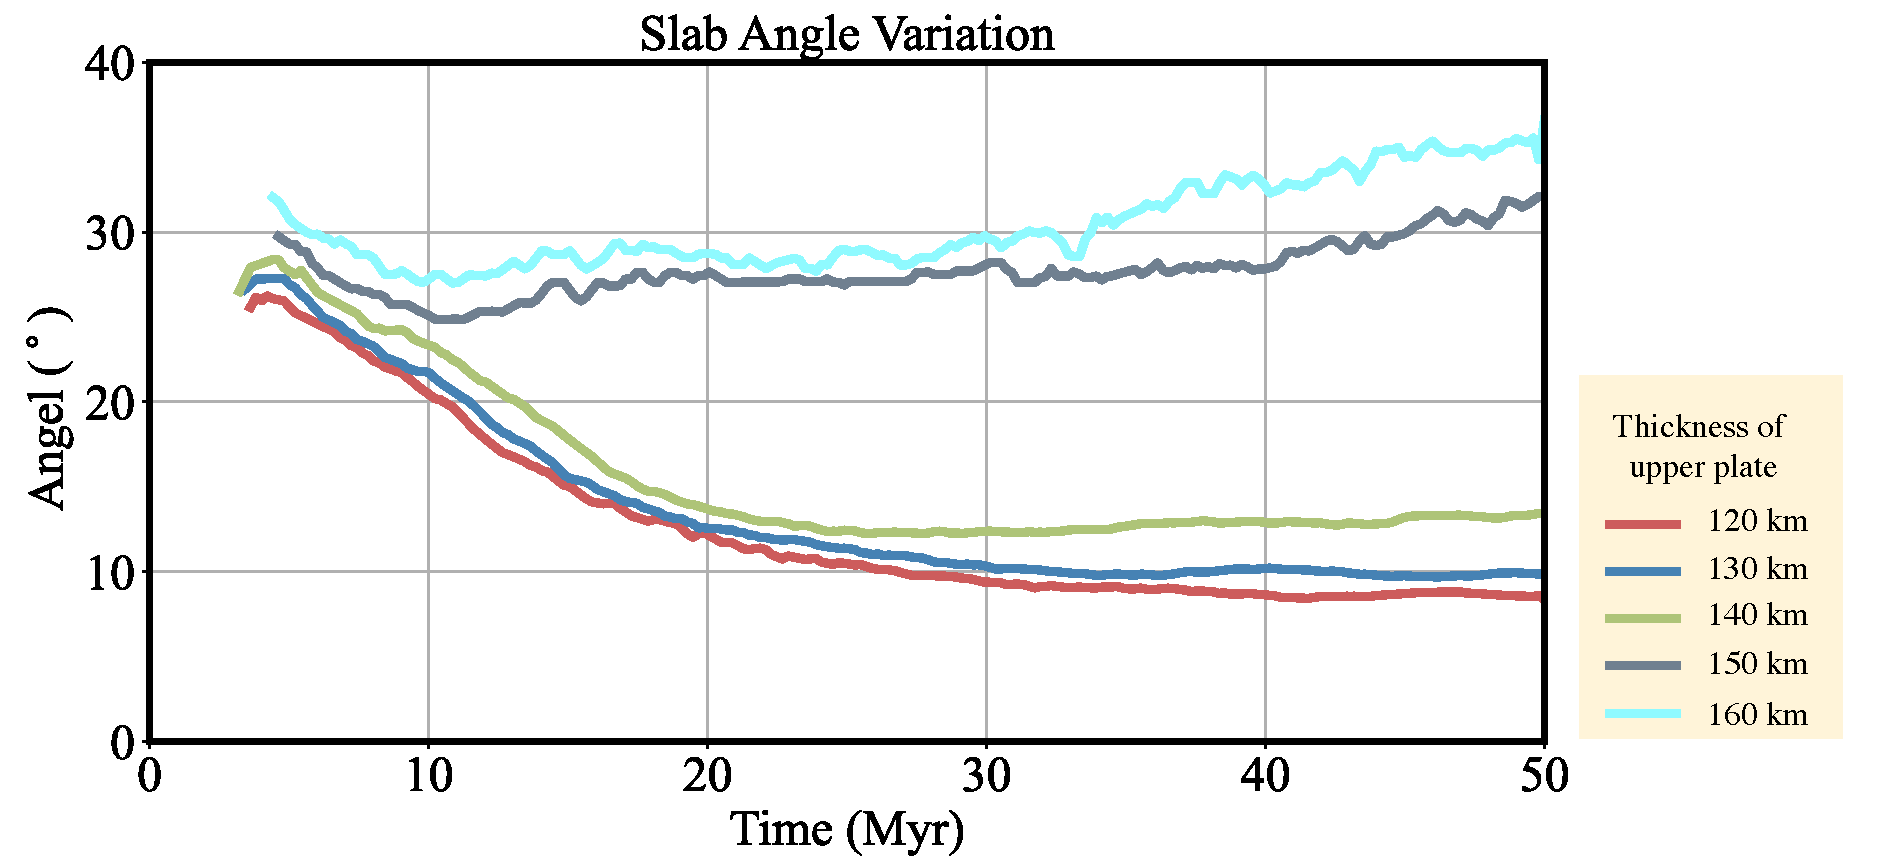
\includegraphics[width=6in]{compare_dip_thermal_Nazca_v2.pdf}
    \caption[測試上覆板塊厚度模型之150公里以上隱沒傾角隨時間變化]{測試上覆板塊厚度模型之150公里以上隱沒傾角隨時間變化。}
    \label{fig::compare_dip_thermal}
\end{figure*}

該結果表明,上覆板塊厚度在140公里以內的隱沒傾角在模型時間20 Myr後可低於15$^\circ$以內,反之,上覆板塊厚度150公里與160公里的模型隱沒傾角在任何時間皆高於25$^\circ$。
若將每個模型的隱沒板塊頂部在相同模型時間內隨深度繪出,可獲得圖\ref{fig::compare_geometry}。
從圖中可見,平坦隱沒特徵僅出現在上覆板塊厚度為120公里、130公里、140公里的三個模型中,而上覆板塊厚度150公里與160公里的兩個模型則是正常傾角的隱沒帶。
這意味著上覆板塊的溫度構造會大程度的影響隱沒板塊的隱沒構造,並且,高溫的環境較容易生成平坦隱沒。
此外,圖\ref{fig::compare_geometry}顯示平坦隱沒的平坦長度與深度在不同模型中有出入,藉由計算模型中平坦段的長度與深度,可獲得圖\ref{fig::compare_slab_time}

\begin{figure*}[ht!]
    \centering
    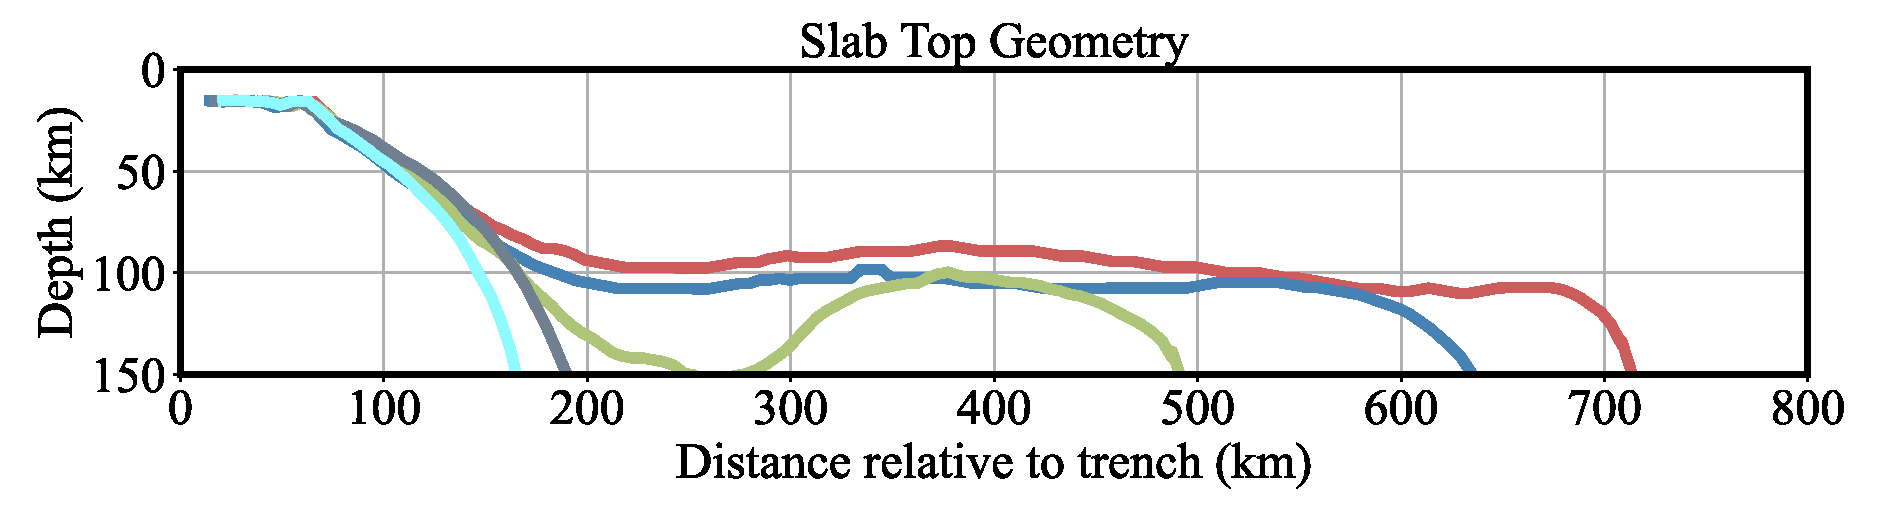
\includegraphics[width=6in]{slab_geometry_thermal_Nazca_v2.pdf}
    \caption[測試上覆板塊厚度模型在40 Myr的隱沒板塊構造]{測試上覆板塊厚度模型在40 Myr時隱沒板塊於150公里以上之構造,幾何形狀取自隱沒板塊頂部,使用5公里移動平均平滑離散化的網格,模型與圖\ref{fig::compare_dip_thermal}所使用的圖例相同。}
    \label{fig::compare_geometry}
\end{figure*}

較高溫的上覆板塊構造會在較淺的深度形成較長的平坦隱沒段,與\ref{智利參考模型結果}節的推測相同,平坦段深度大致與原先大陸岩石圈攝氏 800$^\circ$ 等溫線深度相同,因此較薄的大陸岩石圈有較淺的平坦隱沒段。
三個模型的平坦隱沒段長度差亦可達超過100公里。

\begin{figure*}[ht!]
    \centering
    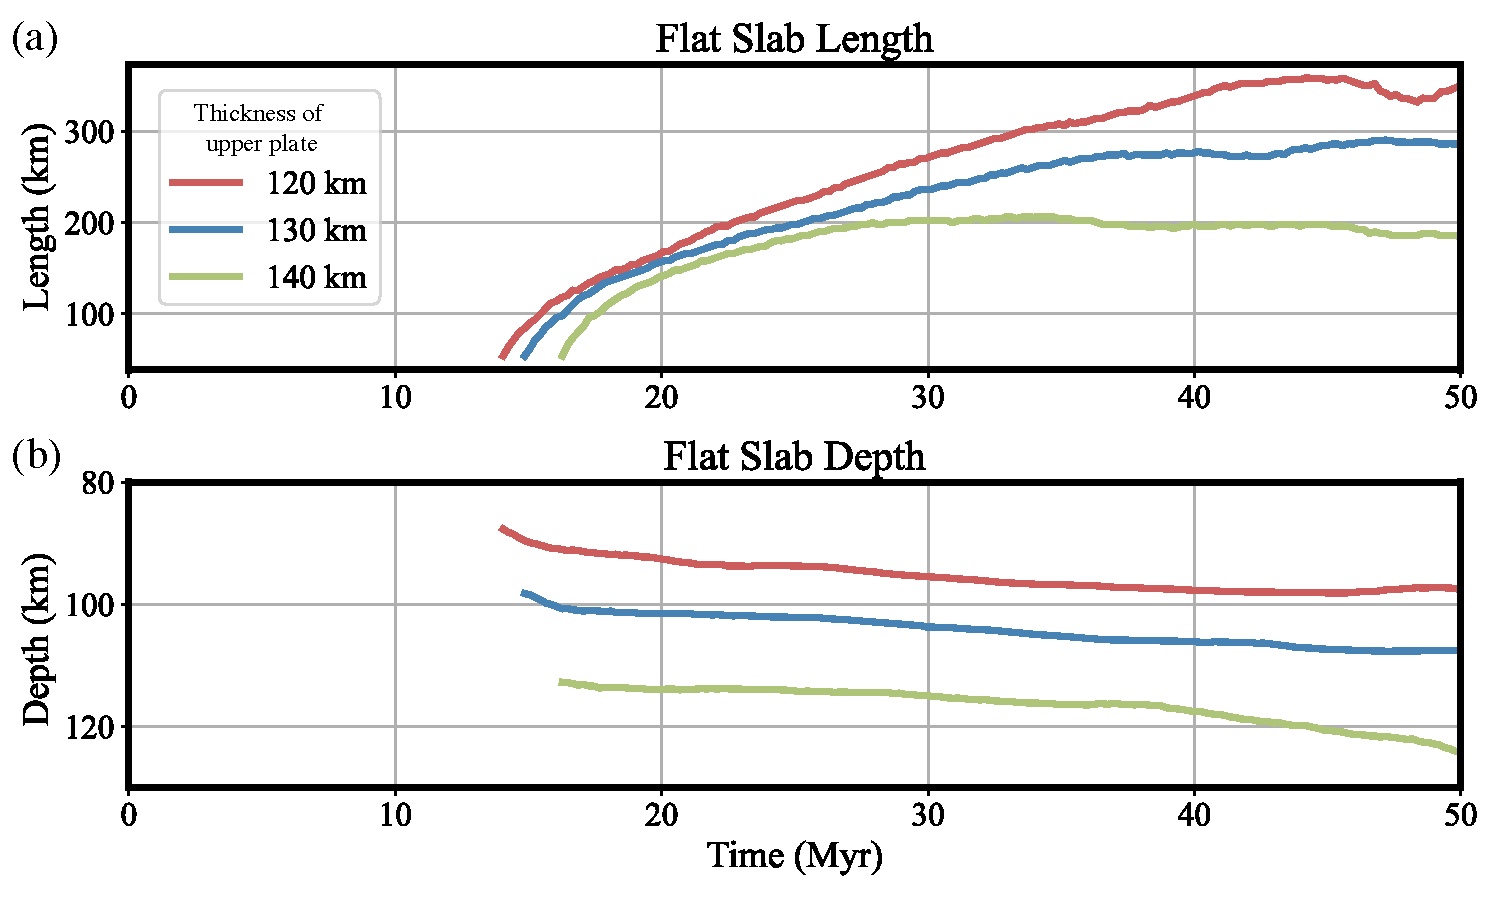
\includegraphics[width=5in]{thermal_Nazca_flatslab_length_v2.pdf}
    \caption[測試上覆板塊厚度模型的平坦段長度與深度]{測試上覆板塊厚度模型的平坦段(a)長度與(b)深度。模型與圖\ref{fig::compare_dip_thermal}所使用的圖例相同。}
    \label{fig::compare_slab_time}
\end{figure*}

這系列上覆板塊測試結果表明,較高溫的上覆板塊較容易形成平坦隱沒。
\citet{liu2019influence}的數值模型利用改變上覆板塊的溫度構造與強度探討平坦隱沒的形成機制,他們的模型使用線性地溫梯度控制上覆板塊最終厚度,固定板塊底部的溫度為攝氏1336$^\circ$,並系統性測試模型中上覆板塊厚度自60-240公里對平坦隱沒的影響。
他們的結果顯示越薄、等深度下溫度越高的上覆板塊會形成深度越淺且長度越長的平坦隱沒段。
儘管他們的研究中,上覆板塊的溫度並不是決定平坦隱沒形成的關鍵因素,然而他們支持較高溫的上覆板塊較容易形成平坦隱沒,這項研究結果與本系列模型相似。
本研究認為,較高溫的大陸岩石圈具有黏滯度較低的岩石流變行為,因此岩石圈強度較低。
冷硬的隱沒板塊可能在大陸岩石圈強度較低的情況下輕易將岩石圈底部推開,形成長度較長的平坦隱沒段。

%他們的模型中,他們的結論表明較薄的上覆板塊比起冷硬的板塊更容易形成平坦隱沒,他們將結果歸因於較熱的上覆板塊具有黏滯度較小的地函岩石圈,進而導致隱沒板塊沿著
%容易促使平坦隱沒行成。

\subsubsection{墨西哥平坦隱沒的上覆板塊}
在墨西哥區域,\citet{Manea2011Curie}曾經利用地磁資料計算墨西哥南部的居禮溫度(Curie temperature)面深度,進而獲得隱沒帶區域的溫度構造觀測資料。
在他們的研究中,針對兩條垂直於海溝的剖面進行討論,一條剖面為平坦隱沒段,另一條剖面為正常隱沒段。

平坦隱沒剖面在弧後區域具有較淺的居禮溫度面,由地磁獲得的估計居禮溫度面在弧後區深度約20-25公里,由他們研究中的熱模型推得的居禮溫度面深度約30公里左右,本研究墨西哥參考模型初始穩定大陸的居禮溫度面深度為28.5公里。

正常隱沒剖面的居禮溫度面範圍較大,地磁資料的結果落在15-30公里不等,不過他們的熱模型結果表示居禮溫度面在弧後區約落在42公里左右(見圖\ref{fig::Curie_Point_model})。
比較\citet{Manea2011Curie}中的熱模型與本研究模型結果,測試一組居禮溫度面為38公里的初始墨西哥模型。
該模型在40公里前淺部地溫梯度為每公里攝氏15$^\circ$,而參考模型的地溫梯度為每公里攝氏20$^\circ$。

\begin{figure*}[ht!]
    \centering
    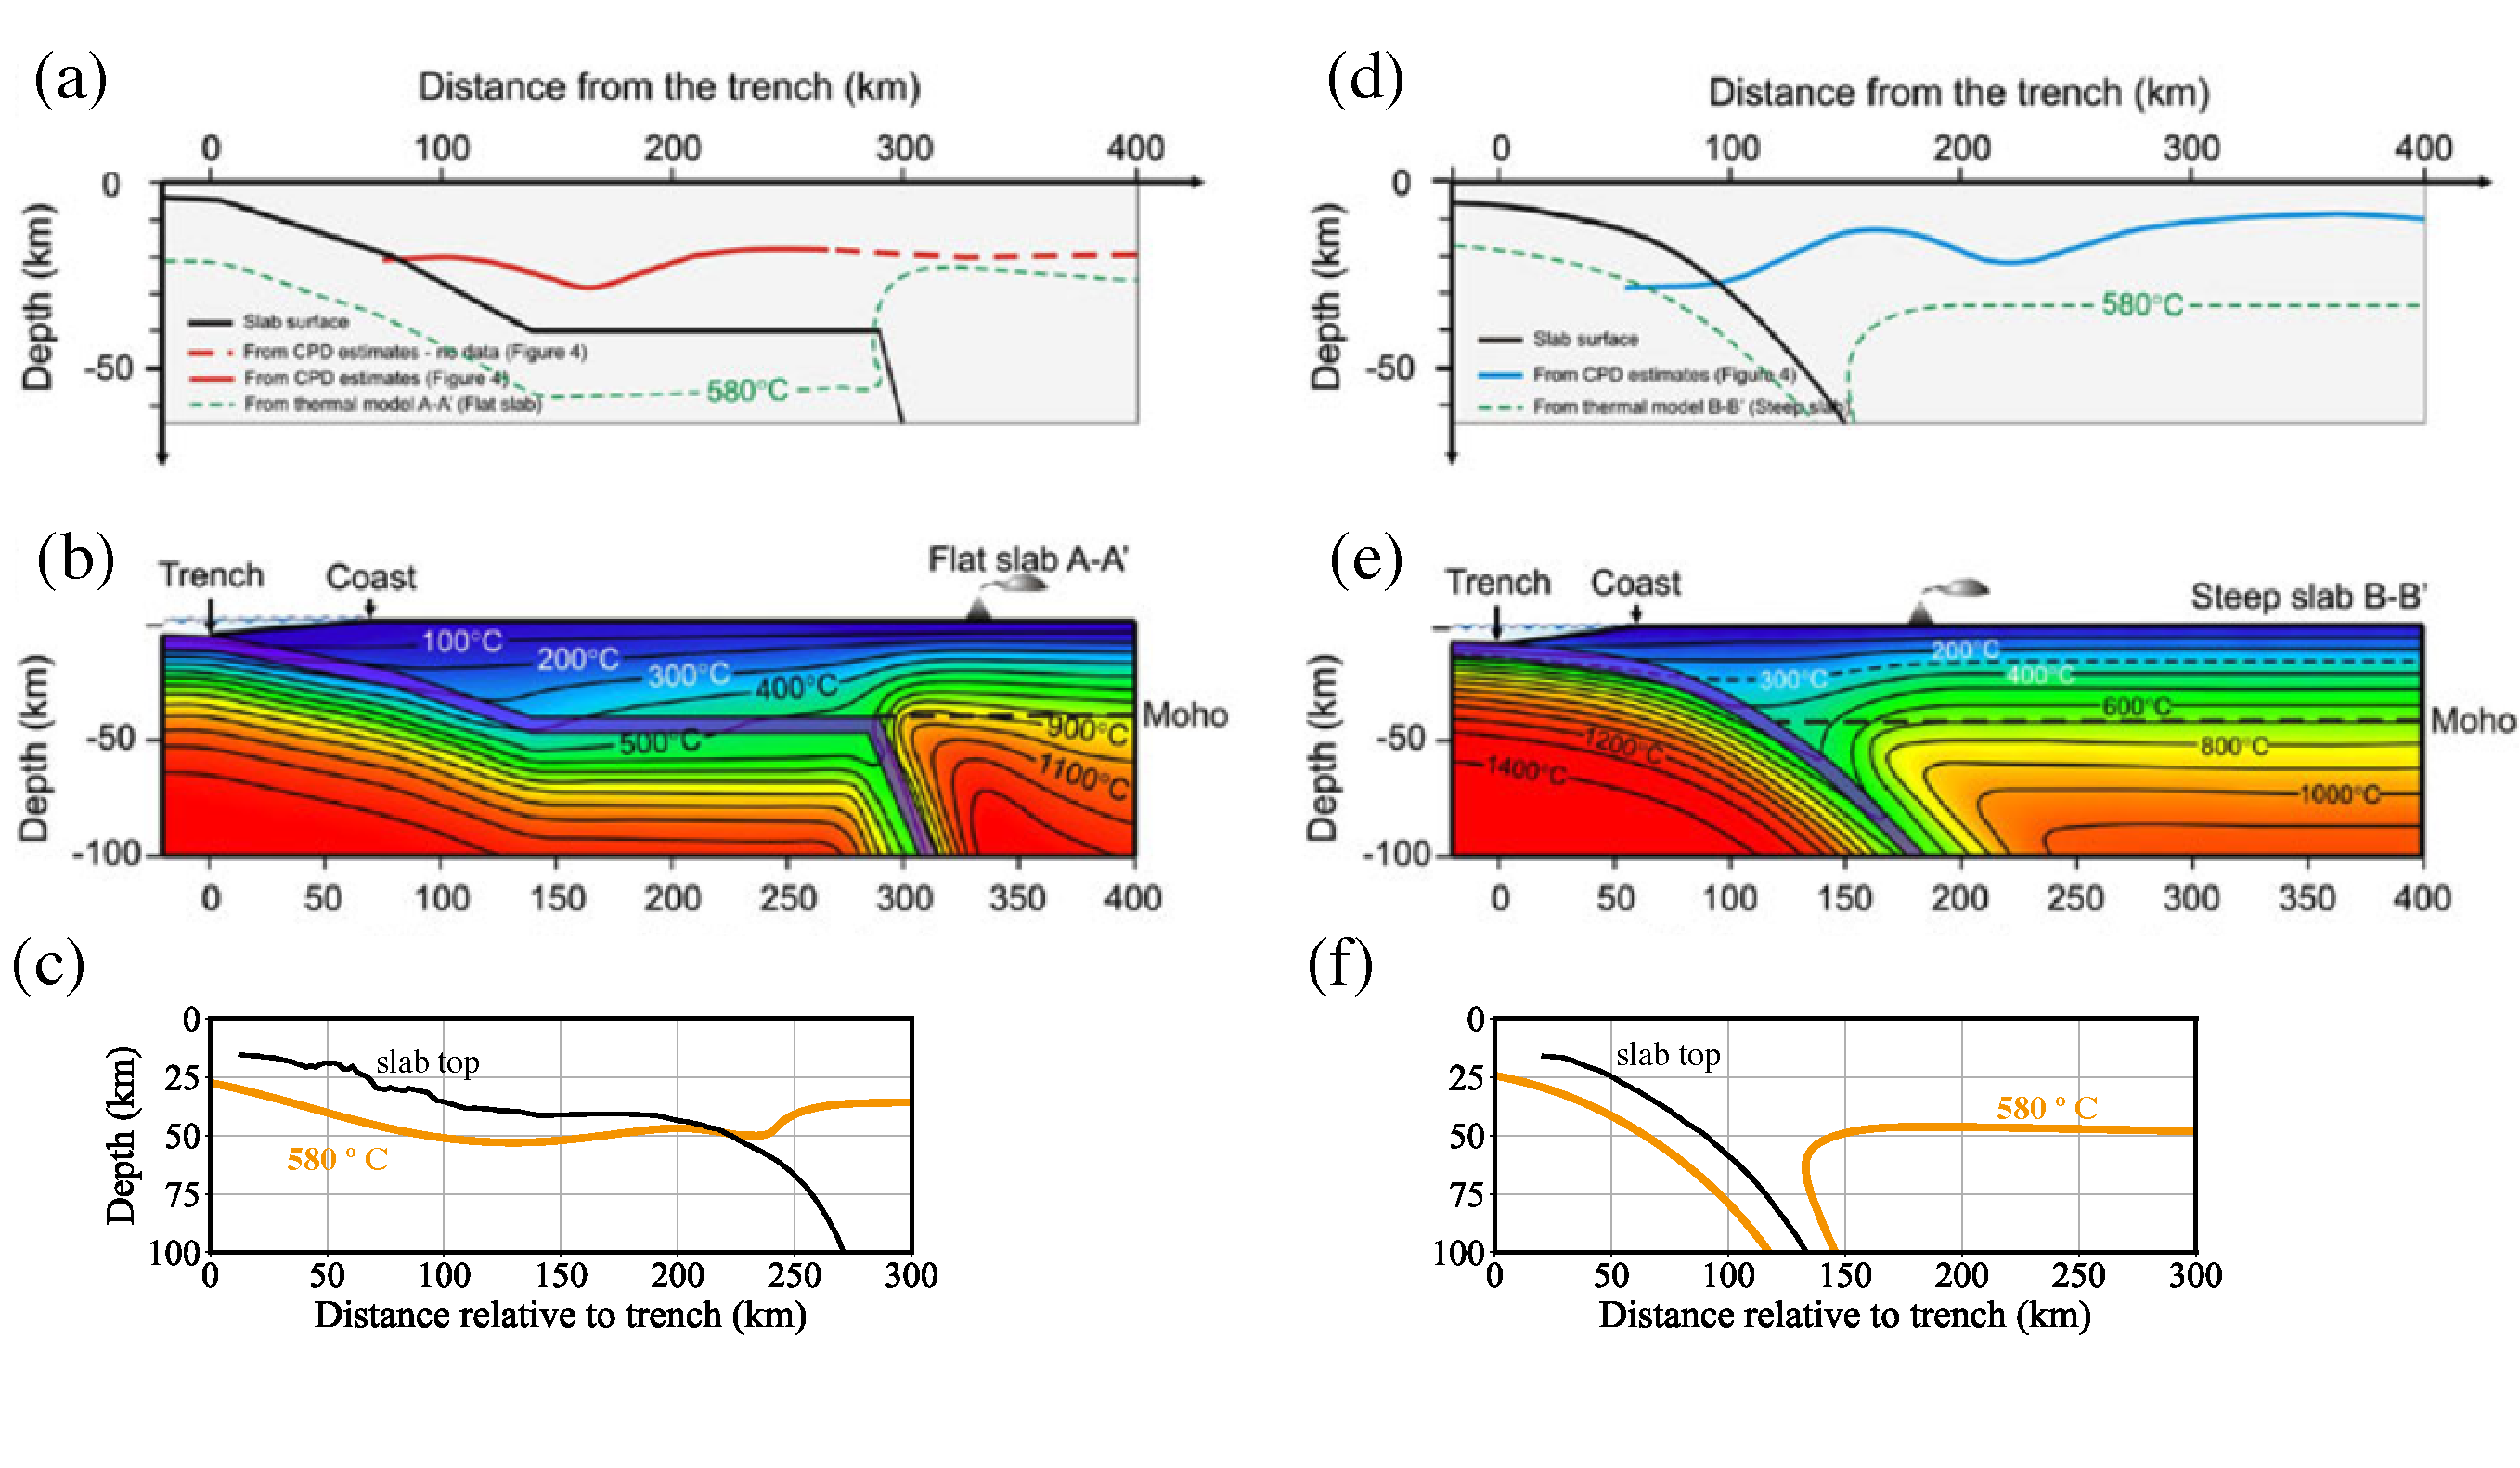
\includegraphics[width=6in]{CurieMexico_v3.pdf}
    \caption[墨西哥兩條剖面的居禮溫度面與熱構造模型與不同地溫梯度的墨西哥模型在30 Myr的隱沒板塊構造與580$^\circ$等溫線]{(a)(b)(d)(e)墨西哥兩條剖面的居禮溫度面與熱構造模型,摘自\citet{Manea2011Curie}。(c)(f)不同地溫梯度的墨西哥模型在30 Myr的隱沒板塊構造(黑線)於100公里以上之剖面與580$^\circ$等溫線(橘線),幾何形狀取自隱沒板塊頂部,使用5公里移動平均平滑離散化的網格。(a)繪出平坦隱沒區域的居禮溫度面(紅線,虛線為外差值)、隱沒板塊頂部(黑線)與\citet{Manea2011Curie}中熱模型攝氏580$^\circ$等溫線。(b)\citet{Manea2011Curie}的平坦隱沒熱模型。(c)墨西哥參考模型在30 Myr的隱沒板塊構造(黑線)於100公里以上之剖面與580$^\circ$等溫線(橘線)。(d)繪出正常隱沒區域的居禮溫度面(藍線)、隱沒板塊頂部(黑線)與\citet{Manea2011Curie}中熱模型攝氏580$^\circ$等溫線。(e)\citet{Manea2011Curie}的正常隱沒熱模型。(f)測試一組於地表至40公里中每公里攝氏15$^\circ$的模型。模型於30 Myr的隱沒板塊構造(黑線)於100公里以上之剖面與580$^\circ$等溫線(橘線)。
    }
    \label{fig::Curie_Point_model}
\end{figure*}

圖\ref{fig::Curie_Point_model}顯示與\citet{Manea2011Curie}類似的居禮溫度面結果,並且,與智利參考模型的結論相似,較高溫的大陸岩石圈較容易產生平坦隱沒。
本研究認為,儘管較高的岩石圈溫度會導致地函黏滯度降低,進而降低作用在隱沒板塊上的動水壓力,然而溫度升高同時導致岩石圈強度下降,此時隱沒板塊容易將弱的地函岩石圈推開,促使平坦隱沒發育。

\newpage
\subsection{地函楔中的動水壓力力矩}
由於本研究中,只有智利參考模型的平坦隱沒上方包含地函楔,因此本節僅會測試與討論智利參考模型。
\citet{Manea2007}與\citet{Yan2020}提及隱沒帶脫水作用應是對動水壓力力矩有重大影響的因素之一。
大量的脫水會降低地函楔黏滯度與地函岩石強度,因此可能會降低地函動水壓力力矩的量值。
除了脫水作用外,岩漿作用也是另一個會影響地函楔黏滯度與岩石強度的因素(\citealp{jamieson2011crustal})。
在模型中,當地函楔發生部分熔融後,岩漿庫所產生的潛熱造成地函楔局部溫度增加,進而降低地函楔的黏滯度。
過去的數值模型鮮少討論岩漿作用對隱沒系統的動水壓力力矩影響,因此本研究對岩漿參數做一系列測試,用以探討兩者的關聯。
本節會先利用蛇紋岩厚度測試脫水作用對動水壓力力矩的影響,再討論岩漿作用與動水壓力力矩的關係。

\subsubsection{隱沒帶的脫水作用}
本研究數值模型的蛇紋岩產生量可自由控制(見\ref{蛇紋岩化的橄欖岩}節),本研究中,與普通橄欖岩相比,蛇紋岩具有較低的活化能(\citealp{hilairet2007high}),並約略等同於欖岩中有15$\%$之橄欖岩被蛇紋岩化。
模型中蛇紋岩的厚度可是為隱沒帶中脫水作用的活躍度,越厚的蛇紋岩可視為越劇烈的脫水環境。
因此本研究利用測試隱沒系統中不同蛇紋岩厚度探討脫水作用對智利參考模型的影響。
受限於網格解析度,因此測試厚度為2.5公里、5公里、7.5公里、10公里與15公里,每個模型的參數見表\ref{模型參數列表}b。
若將每個模型的隱沒板塊頂部在相同模型時間內隨深度繪出,可獲得圖\ref{fig::slab_geometry_serpentinite_thickness_Nazca_top}。

\begin{figure*}[ht!]
    \centering
    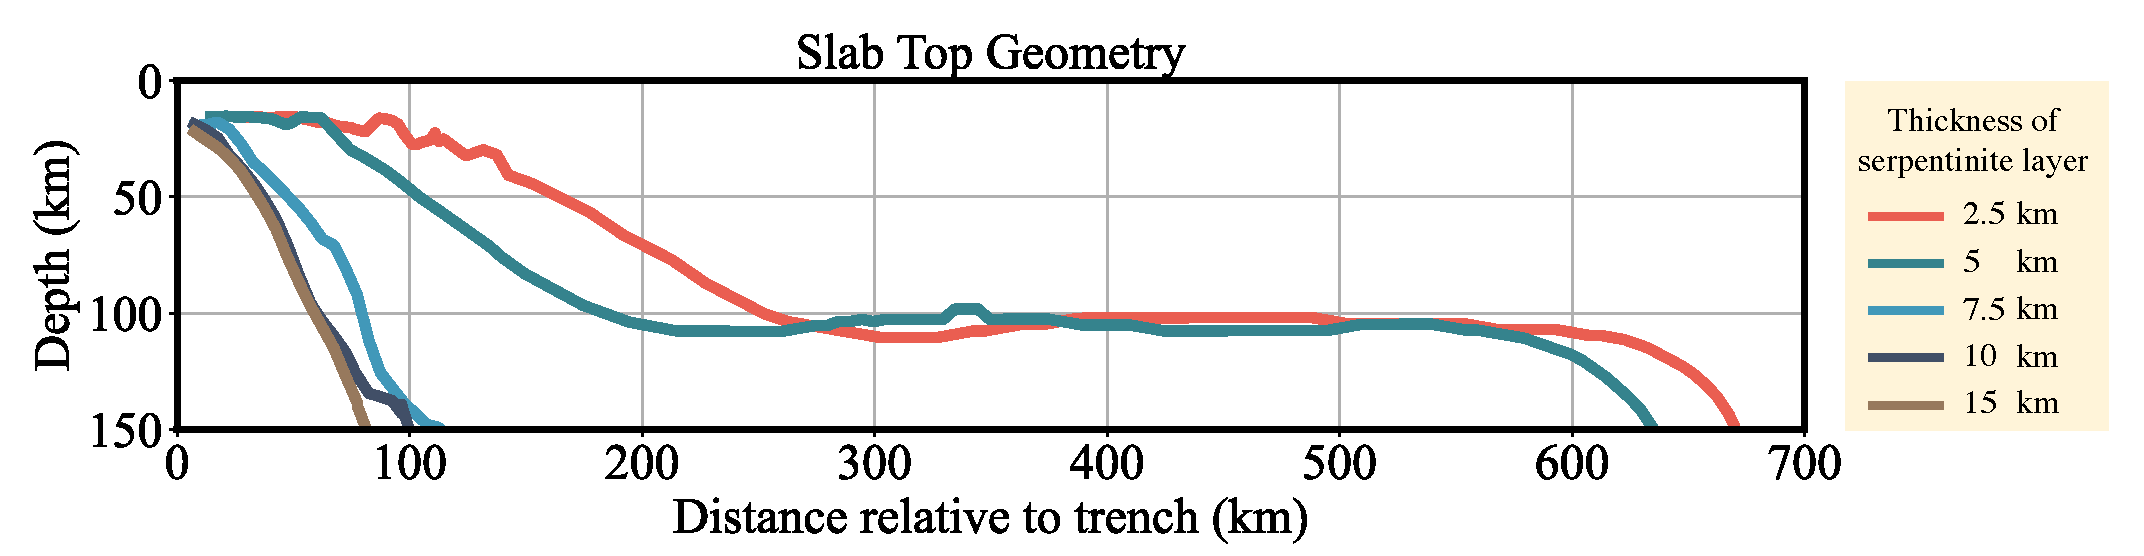
\includegraphics[width=5in]{slab_geometry_serpentinite_thickness_Nazca_v2.pdf}
    \caption[測試蛇紋岩厚度模型的隱沒板塊頂部剖面圖]{測試蛇紋岩厚度模型的隱沒板塊頂部剖面圖,使用5公里移動平均平滑離散化的網格。}
    \label{fig::slab_geometry_serpentinite_thickness_Nazca_top}
\end{figure*}

結果表明,只有蛇紋岩厚度為2.5公里與5公里的模型為平坦隱沒,亦即較活躍的脫水作用不容易形成平坦隱沒。
本系列模型之動水壓力力矩隨時間變化圖(圖\ref{fig::serpentinite_thickness_Nazca_suction})可見兩者的動水壓力力矩於10 Myr後開始呈現兩極化,蛇紋岩厚度為2.5公里與5公里的模型動水壓力力矩在10 Myr後快速增加。
從圖\ref{fig::serpentinite_thickness_Nazca_compare_viscosity}c來看,地函楔中的低壓帶於10 Myr後形成,是動水壓力力矩的增加主因。
反觀蛇紋岩厚度超過5公里的模型,動水壓力力矩在10 Myr之後便趨近於0,因此模型無法形成平坦隱沒。
圖\ref{fig::serpentinite_thickness_Nazca_compare_viscosity}d中顯示蛇紋岩厚度為7.5公里的模型動水壓力剖面,儘管模型在10 Myr有地函楔低壓帶存在,然而於12 Myr前後地函楔壓力明顯高於蛇紋岩厚度5公里的模型(圖\ref{fig::serpentinite_thickness_Nazca_compare_viscosity}c),隨後至14 Myr,地函楔低壓帶已逐漸與周遭地函平衡。
圖\ref{fig::serpentinite_thickness_Nazca_compare_viscosity}b是蛇紋岩厚度為7.5公里的模型的黏滯度剖面,可見軟流圈在12 Myr後進入原先地函楔低壓區,此時,隱沒板塊上下的壓力差趨近於0,動水壓力力矩降低。

\begin{figure*}[ht!]
    \centering
    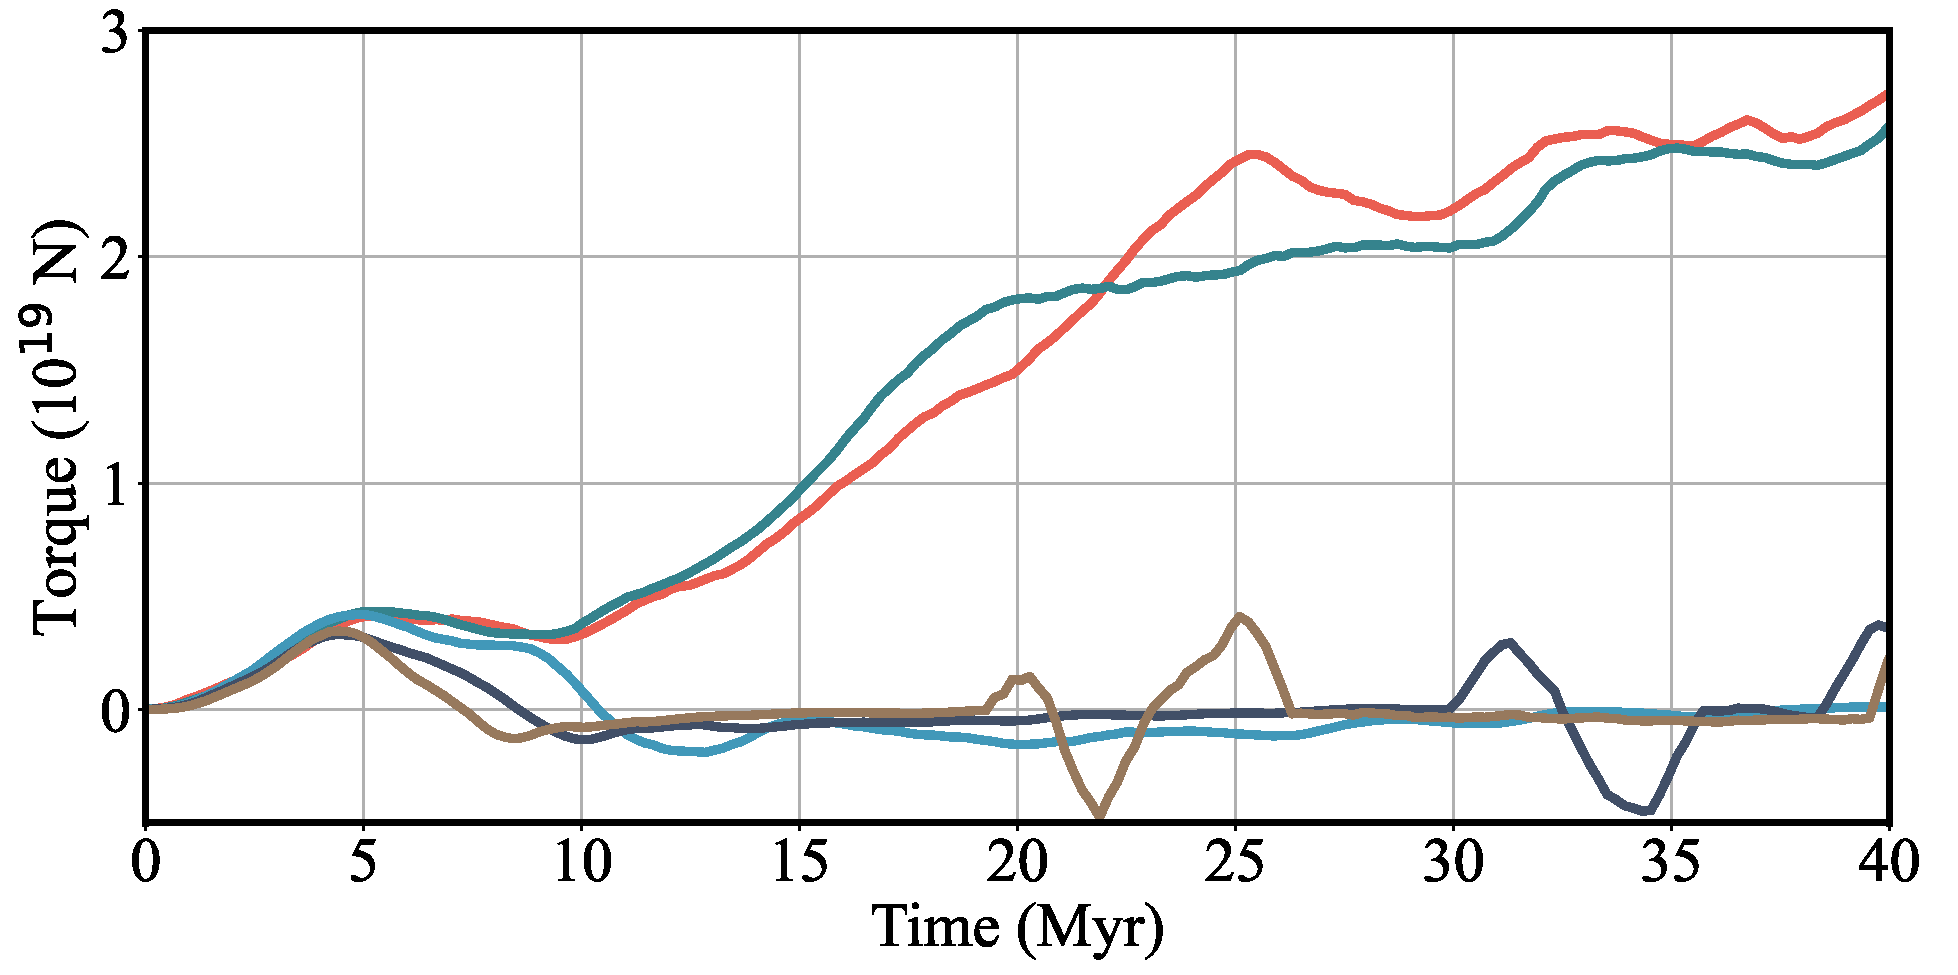
\includegraphics[width=5in]{serpentinite_thickness_Nazca_suction_v1.pdf}
    \caption[測試蛇紋岩厚度模型之動水壓力力矩]{測試蛇紋岩厚度模型之動水壓力力矩,模型與圖\ref{fig::slab_geometry_serpentinite_thickness_Nazca_top}所使用的圖例相同。}
    \label{fig::serpentinite_thickness_Nazca_suction}
\end{figure*}

從模型中的黏滯度剖面圖\ref{fig::serpentinite_thickness_Nazca_compare_viscosity}可見板塊交界處有一細窄低黏滯度通道,假設低黏滯度通道的寬度為隱沒板塊與上覆板塊之間黏滯度低於10$^{21}$ Pa$\cdot$s的寬度。
兩個模型間的低黏滯度通道在模型時間10 Myr表現出可辨別的寬度差,在這裡為蛇紋岩厚度的影響。
相對於地函岩石圈中的低壓環境,地函岩石圈中的軟流圈動水壓力較大,較厚的低黏滯度通道導致溫暖的軟流圈容易藉由壓力差流入板塊交界處中,
一旦低黏滯度通道與軟流圈相互連結,地函流容易流入地函岩石圈,促使隱沒板塊交界處形成一開放系統。
此時,地函岩石圈中原先的低壓環境隨著地函流的流入而被平衡,動水壓力隨後趨近於0,可見圖\ref{fig::serpentinite_thickness_Nazca_compare_viscosity}中10-14 Myr間動水壓力的變化。

\begin{figure*}[htp!]
    \centering
    \includegraphics[width=6in]{serpentinite_compare_Nazca_v1.pdf}
    \caption[測試蛇紋岩厚度模型於5 Myr、10 Myr、12 Myr與14 Myr之黏滯度與動水壓力剖面]{測試蛇紋岩厚度模型於5 Myr、10 Myr、12 Myr與14 Myr之黏滯度與動水壓力剖面。(a)蛇紋岩厚度為5公里的模型黏滯度剖面。(b)蛇紋岩厚度為7.5公里的模型黏滯度剖面。(c)蛇紋岩厚度為5公里的模型動水壓力剖面。(d)蛇紋岩厚度為7.5公里的模型動水壓力剖面。}
    \label{fig::serpentinite_thickness_Nazca_compare_viscosity}
\end{figure*}

\newpage
\subsubsection{隱沒帶的岩漿作用}
本研究數值模型岩漿作用與多個參數有關,控制著岩漿庫的增加速率與冷卻速率,詳細方法可見\ref{岩漿作用}節。
為了瞭解岩漿作用對隱沒系統的影響,本研究測試岩漿產生速率P$_{m0}$與岩漿冷卻衰變常數$\lambda_{m0}$分別為P$_k$與$\lambda_k$的倍數,獲得共12個模型,其中P$_k$=4.5$\times$10$^{-13}$,$\lambda_k$=1.6$\times$10$^{-12}$。
詳細的模型參數可見表\ref{模型參數列表}與圖\ref{fig::magma parameter}。

\begin{figure*}[ht]
    \centering
    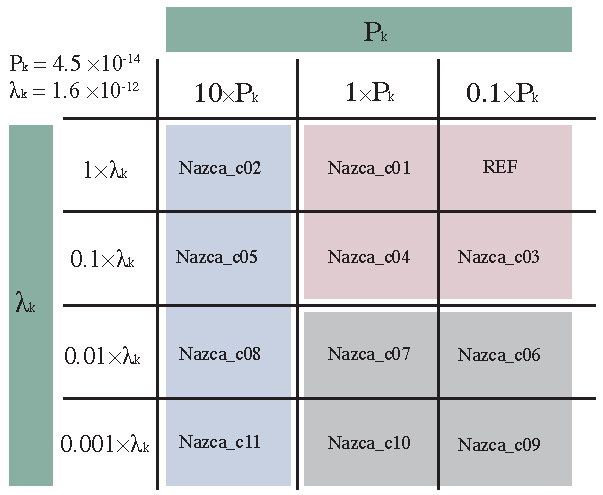
\includegraphics[width=4in]{magma parameter.pdf}
    \caption[智利模型岩漿參數測試示意圖,詳細岩漿參數見表\ref{模型參數列表}]{智利模型岩漿參數測試示意圖,詳細岩漿參數見表\ref{模型參數列表}。底部顏色為圖\ref{fig::magma_area_compare_Nazca}中的說明顏色。}
    \label{fig::magma parameter}
\end{figure*}

這系列模型結果顯示兩極化的隱沒板塊幾何狀態,可分為具有平坦隱沒的模型與正常隱沒模型。
若將每個模型的隱沒板塊頂部隨深度繪出,可獲得圖\ref{fig::magma_area_compare_Nazca}a。
圖中藍線則為此系列模型中正常隱沒模型的隱沒板塊頂部,隱沒板塊的幾何曲線幾何形狀趨近於一致。
紅線與黑線為此系列模型中具有平坦隱沒特徵的隱沒板塊頂部,平坦隱沒的深度並沒有明顯變化,不過隱沒板塊的曲線又可約略被分為兩群。
紅線群為平坦段斜率變化較小的一群模型,反之為黑線群。
紅線群包含岩漿冷卻衰變常數$\lambda_{m0}=1.6\times 10^{-12}$與$\lambda_{m0}=1.6\times 10^{-13}$,而黑線包含岩漿冷卻衰變常數$\lambda_{m0}=1.6\times 10^{-14}$與$\lambda_{m0}=1.6\times 10^{-15}$。
該結果可能可以為平坦隱沒在部分區域有強烈曲率變化提供一可能的影響原因。
秘魯區域的平坦隱沒南段具有劇烈的斜率變化(見圖\ref{fig::Peru_tomography}),\citet{Ma2015}的接收函數研究發現該劇烈曲率變化與莫荷面深度平行,因此他們認為可能是地函岩石圈中強烈的動水壓力對隱沒板塊造成影響。
智利平坦隱沒板塊在平坦段並沒如此劇烈的斜率變化。

在這組參數測試中,岩漿產生速率很大程度上影響岩漿庫的體積大小,岩漿產生速率(P$_{m0}$)越大,則岩漿庫的體積越大。
而岩漿冷卻衰變參數則控制岩漿庫生成後體積量的維持時間,岩漿冷卻參數越大,則岩漿冷卻速度越快,岩漿庫體積越快減少。
岩漿庫體積量隨時間變化之結果如圖\ref{fig::magma_area_compare_Nazca}b。

\begin{figure*}[ht!]
    \centering
    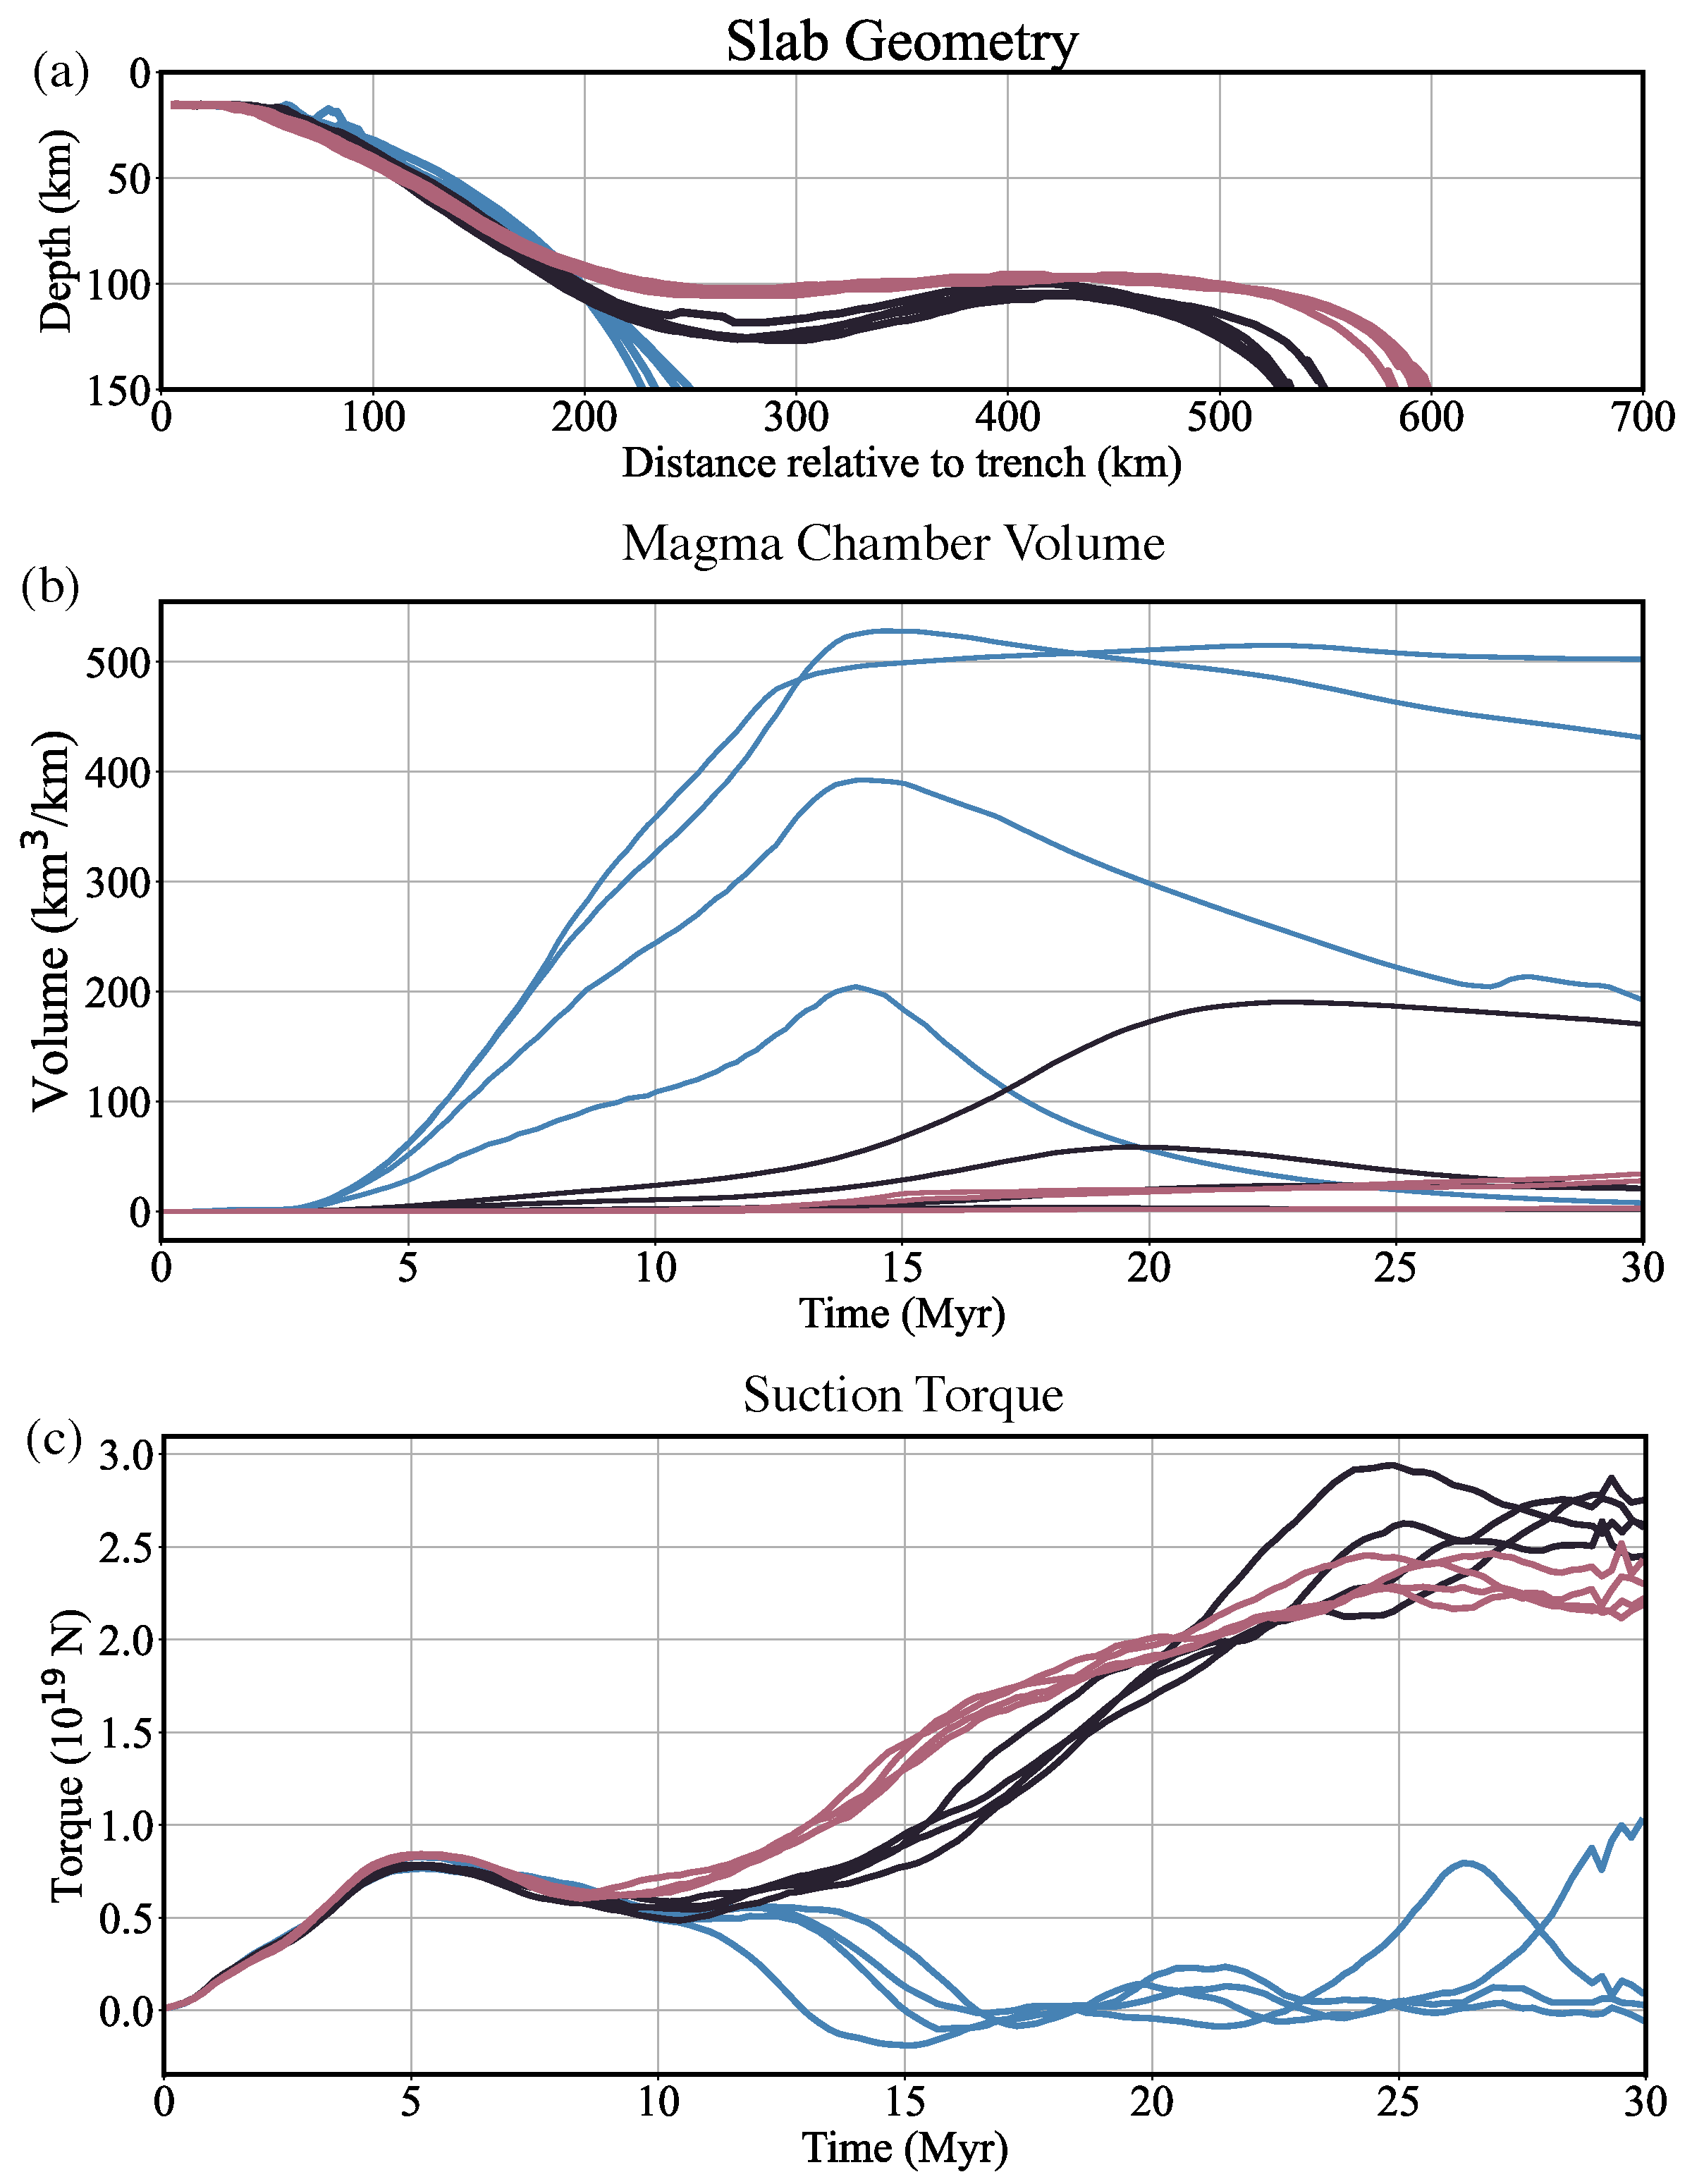
\includegraphics[width=5in]{magma_area_compare.pdf}
    \caption[智利模型岩漿參數測試結果,詳細岩漿參數見表\ref{模型參數列表}與圖\ref{fig::magma parameter}]{智利模型岩漿參數測試結果,詳細岩漿參數見表\ref{模型參數列表}與圖\ref{fig::magma parameter}。圖中不同線條(模型間)的顏色分類與圖\ref{fig::magma parameter}相同,共將模型分成三群。(a)隱沒板塊幾何形狀。(b)所有模型岩漿庫體積隨時間變化。(c)所有模型動水壓力力矩隨時間變化。}
    \label{fig::magma_area_compare_Nazca}
\end{figure*}

當岩漿產生速率為10 P$_k$ (P$_{m0}$ =4.5$\times$10$^{-13}$)時,岩漿庫體積在5 Myr後開始顯著增加,並且在15 Myr前岩漿庫體積達到最高峰。
一旦模型中的岩漿庫在15 Myr年之前體積超過200 km$^3$/km,則模型變會成為一正常隱沒帶,而非平坦隱沒。
因此岩漿庫的體積可能會影響地函中的動水壓力力矩。
動水壓力力矩隨時間變化結果如圖\ref{fig::magma_area_compare_Nazca}c,動水壓力力矩在15 Myr前後呈現兩極化,在岩漿產生速率P$_{m0}$=4.5$\times$10$^{-13}$的模型中,動水壓力力矩皆快速下降。

岩漿於冷卻過程中會釋放潛熱,導致地函楔中溫度升高。
而由於溫度與黏滯度有高度相關性,因此,越大量的岩漿體積會導致地函溫度較高,進而降低地函黏滯度,
與脫水作用的影響相同,地函岩石圈中若具有較低的黏滯度,容易促成溫暖的軟流圈與地函楔相連結,
又因為相對於地函楔中原先的低壓環境,軟流圈動水壓力較高,因此一旦岩石黏滯度夠低,軟流圈地函流可輕易上湧進入板塊交界處中。
地函流流入地函岩石圈後,地函楔的低壓環境逐漸消失,因此施加於隱沒板塊上的動水壓力矩變低,隱沒系統不容易形成平坦隱沒。

這系列模型中可初步說明,岩漿作用有可能會大程度地減少隱沒帶的動水壓力,與隱沒帶脫水作用所扮演的角色相同。
早期地函動力學中計算隱沒系統之解析解認為作用在隱沒板塊上的吸力極大,因此判斷地球早期大部分的隱沒系統皆為平坦隱沒(\citealp{tovish1978mantle}; \citealp{vlaar1983thermal}; \citealp{abbott1994flat})。
隨著地震站的廣設,現今全球隱沒板塊模型(\citealp{hayes2018slab2})顯示平坦隱沒並不常見於現今隱沒帶。
近年來數值模型表明地函吸力在早期被低估,隱沒板塊的脫水與地函楔的水合作用會產生低黏滯度地函楔,大幅降低地函吸力,因此真實的地函吸力應遠低於過去認知(\citealp{Manea2007})。
地函的動水壓力與地函中的溫度、壓力、岩石強度等性質有關,除了脫水作用外,本研究認為岩漿作用可能是另一個影響地函動水壓力的主要作用。


\section{本研究的不足之處}

1. 近年來的研究支持平坦隱沒可能與隱沒板塊與660不連續面的交互作用有關(\citealp{chen2019southward}; \citealp{schellart2020control}; \citealp{Schellart2021}),然而本研究智利參考模型僅300公里,無法參與這部分的討論。

2. 在智利參考模型中,平坦隱沒的特徵在隱沒早期便出現,亦即該模型並不是從一正常傾角的隱沒帶漸演化成平坦隱沒。
現生納茲卡隱沒帶已存在超過150 Ma,中間曾經經歷重新隱沒(\citealp{chen2019southward}; \citealp{hu2021southward}),平坦隱沒的發育時間約從8 Myr前後開始,更早期的隱沒板塊應為正常傾角。
然而本研究並無法重現自高角度隱沒帶到平坦隱沒的演化。

3. 本研究目前只能提供影響動水壓力的因素,但無法量化其影響動水壓力的量值。
